\documentclass[12pt,a4paper,openright,twoside]{book}
\usepackage[utf8]{inputenc}
\usepackage{disi-thesis}
\usepackage{code-lstlistings}
\usepackage{notes}
\usepackage{shortcuts}
\usepackage{csquotes}
\usepackage{acronym}

\school{\unibo}
\programme{Corso di Laurea Magistrale in Ingegneria e Scienze Informatiche}
\title{Design and implementation of a scalable domain specific language foundation for ScaFi with Scala 3}
\author{Luca Deluigi}
\date{\today}
\subject{Paradigmi di Programmazione e Sviluppo}
\supervisor{Prof. Mirko Viroli}
\cosupervisor{Dott. Gianluca Aguzzi}
% \morecosupervisor{Dott. Roberto Casadei}
\session{IV}
\academicyear{2022-2023}

% Definition of acronyms
\acrodef{IoT}{Internet of Thing}
\acrodef{VM}{Virtual Machine}
\acrodef{CAS}{Collective Adaptive System}
\acrodef{MAS}{Multi Agent System}
\acrodef{DSL}{Domain Specific Language}
\acrodef{FC}{Field Calculus}
\acrodef{HFC}{Higher-Order Field Calculus}
\acrodef{XC}{Exchange Calculus}
\acrodef{AST}{Abstract Syntax Tree}
\acrodef{ML}{Meta Language}
\acrodef{DOT}{Dependent Object Types}
\acrodef{FP}{Functional Programming}
\acrodef{JS}{JavaScript}
\acrodef{JVM}{Java Virtual Machine}
\acrodef{API}{Application Programming Interface}
\acrodef{SBT}{Simple Build Tool}
\acrodef{MoSCoW}{Must, Should, Could, Won't}
\acrodef{GUI}{Graphical User Interface}
\acrodef{UML}{Unified Modeling Language}
\acrodef{ADT}{Abstract Data Type}

% Definition of math operators
\DeclareMathOperator{\return}{return\,}
\DeclareMathOperator{\send}{\:send\,}
\DeclareMathOperator{\retsend}{retsend\,}

\mainlinespacing{1.241} % line spacing in mainmatter, comment to default (1)

\begin{document}

\frontmatter\frontispiece

\begin{abstract}	
Max 2000 characters, strict.
\end{abstract}


\begin{dedication} % this is optional
To my past self who always looked forward to this achievement.
\end{dedication}


% ! TeX root = ../thesis-main.tex
\begin{acknowledgements} % this is optional
\noindent
I would like to thank my supervisor, Professor Mirko Viroli, and his research team, in particular Gianluca Aguzzi and Roberto Casadei, for having supported me and having allowed me to work on this thesis.
%
Thanks for all your time and guidance.

Next, I would like to thank my family, who supported my studies and my choices and accompanied me on this journey.

A special thanks goes to my beloved girlfriend, Giada, who has always been by my side in the past years, supporting and helping me to overcome the difficulties I encountered, and accompanying me in my new life in Rimini.

Finally, I would like to thank all my close friends, with whom I have shared great moments, studying with the \textit{Spaceteam}, playing board games with \textit{Zuga Rèmni}, living the university with \textit{S.P.R.I.Te.}, and working with \textit{EasyDesk}.
%
These names represent the best groups of people I ever met and had the pleasure to pass my time with.
\end{acknowledgements}


%----------------------------------------------------------------------------------------
\tableofcontents   
\listoffigures     % (optional) comment if empty
\lstlistoflistings % (optional) comment if empty
%----------------------------------------------------------------------------------------

\mainmatter

% ! TeX root = ../thesis-main.tex
%----------------------------------------------------------------------------------------
\chapter{Introduction}
\label{chap:introduction}
%----------------------------------------------------------------------------------------

The importance of \acp{CAS} engineering is increasing along with the growing prevalence of large-scale cyber-physical systems, driven by the already pervasive \ac{IoT} and edge computing trends~\cite{collective,pervasive}.
%
\acp{CAS} are a particular subcategory of situated, distributed systems in which a collection of individuals, also called agents, exhibits a non-chaotic behavior characterized by \textit{self-*} properties, such as self-organization, self-healing, and self-configuration.
%
Many of the self-* properties cannot be derived from an individual perspective confined to the behavior of a single agent, but rather they are \textit{emergent} from the complex and dynamic network of interactions within the system and with the environment.
%
As a consequence, obtaining such properties requires a holistic approach to the design and programming of \acp{CAS}, which is not straightforward to achieve with traditional software engineering techniques.

Topologically, \acp{CAS} can be considered a subset of \acp{MAS}, and the programming of their behavior as a whole can be referred to as \textit{Macroprogramming}~\cite{macroprogramming-state-of-the-art}.
%
In the context of macroprogramming, a prominent paradigm is that of \textit{aggregate computing}, where a single program, called the aggregate program, defines the overall behavior of a network of devices or agents~\cite{macroprogramming-state-of-the-art}.
%
Aggregate computing provides benefits to development productivity thanks to four main factors~\cite{scafi}: the \textit{macro-level stance}, which abstracts over low-level details about the individual behavior of agents and their communication media, the \textit{compositionality}, promoting the creation of complex behavior by combining simpler ones, the \textit{formality}, allowing theoretical analyses and formal verification of its properties, and the \textit{practicality}, thanks to the availability of tools supporting programming and simulation of \acp{CAS}.

Among these tools, an in-depth analysis is dedicated to the \textit{ScaFi}, an aggregate programming framework that comprises an internal \ac{DSL} written in Scala 2 with supporting components for simulation, visualization, and execution of aggregate systems, based on the \ac{FC} formal language and computational model~\cite{scafi}.
%
Internal \acp{DSL} are distinguished from external \acp{DSL} by the fact that they are embedded in a host language, such as Scala, and that they exploit the flexibility of their host's syntax to resemble a different language even though they are implemented as libraries.

Recently, a new formal language and computational model called \ac{XC} has been proposed, extending the expressiveness of \ac{FC} while simplifying its set of primitive constructs~\cite{xc}.
%
In the meantime, Scala 2 has been succeeded by Scala 3, which introduces a relevant set of new features and improvements over its predecessor.
%
These two novelties have promoted the development of a new ScaFi, entirely redesigned to be formally based on \ac{XC} and to make the best use of its new host language, Scala 3.
%
That project is the main subject of this thesis.
%
Named \quotes{\this}, it has the ambition to \textit{scale}, meaning to grow with the demand of its user without losing its qualities, such as expressiveness, reusability, maintainability, readability, and performance.


\paragraph{Structure of the Thesis} This thesis first introduces the state of the art in aggregate computing tools and languages.
%
Then, it presents a more in-depth dissertation on \ac{XC} and Scala 3, which are the main theoretical and practical foundations of \this, respectively.
%
In the analysis chapter, the requirements of the project are discussed, followed by the analysis of the current state of the ScaFi framework, from which this project originates.
%
In the design chapter, the architecture of the \texttt{core} module of \this is presented, along with the design choices that have been made for the supportive modules such as \texttt{simulator} and \texttt{tests}.
%
Implementation details are then explained in the following chapter, along with experimental and exploratory developments.
%
The evaluation chapter presents results from the testing and validation of the project, including techniques employed for code quality and maintainability.
%
Finally, the thesis concludes with a discussion of the results and the future work that can be done to improve the project.


% ! TeX root = ../thesis-main.tex
%----------------------------------------------------------------------------------------
\chapter{State of the art}
\label{chap:state-of-the-art}
%----------------------------------------------------------------------------------------

In the field of aggregate programming\cite{aggregate-programming}, multiple frameworks, tools, and experiments have been developed and made available as public resources to support a wide variety of use cases, using different languages and design approaches.
%
Among the state-of-the-art tools in this field are \textit{ScaFi}\footnote{\url{https://github.com/scafi/scafi}}\cite{scafi}, \textit{Protelis}\footnote{\url{https://github.com/Protelis/Protelis}}\cite{protelis}, and \textit{FCPP}\footnote{\url{https://github.com/fcpp/fcpp}}\cite{fcpp} which have been briefly described in their fundamental characteristics in this chapter, with a particular emphasis on ScaFi, of which \this is a redesign and reimplementation.
%
Each of the mentioned libraries is backed by a robust, coherent theoretical foundation, that provides consistency and guarantees the emergence of global properties in derived \acp{CAS}.
%
The theoretical framework that serves as the basis for all cited implementations is the \ac{FC}\cite{fc}, specifically its higher-order version, the \ac{HFC}\cite{hofc}.
%
\ac{FC}, as well as its variants, is a type-safe, formal language for aggregate programming\cite{fc, from-dc-to-fc-and-ap} presented with its operational and denotational semantics, respectively describing the local and global interpretation of field expressions\cite{from-dc-to-fc-and-ap}.
%
From a developer perspective, the key aspect of \ac{FC} is the possibility of focusing on the denotational semantics of field constructs, abstracting away from the local interpretation of expressions and implementation of the constructs.
%
In recent years, a new formal language called \ac{XC}\cite{xc} has been developed, which is a promising evolution of \ac{FC}.
%
\ac{XC}\cite{xc} has the potential to supersede \ac{FC} entirely since it is a simpler yet more expressive language that can be used to implement all the \ac{FC} constructs while retaining their original semantics.
%
\this and FCPP in its current version are based on this newer formal language, further described in \cref{chap:background}, where \ac{FC} and \ac{XC} are briefly compared.
%
Some additional experiments with the implementation of \ac{XC} already exist, such as \textit{imperative-xc}\footnote{\url{https://github.com/cric96/imperative-xc}} and \textit{XC: Scala DSL Implementation}\footnote{\url{https://github.com/scafi/artifact-2021-ecoop-xc}}\cite{xc-experiment-with-scafi}, with the latter described in \cref{chap:state-of-the-art->sec:xc-experiment}.

\section{Protelis} \label{chap:state-of-the-art->sec:protelis}

Protelis is an external domain-specific language derived from the discontinued \textit{Proto}, whose syntax resembles that of C or Java.
%
However, Protelis is purely functional, albeit dynamically typed, and uses a virtual machine written in Java\cite{protelis} for interpretation.
%
As an external \ac{DSL}, Protelis syntax is close to the \ac{FC} language it implements, which distinguishes it from internal \acp{DSL} like ScaFi and FCPP.
%
As a result, domain branching in Protelis is more transparent in its conditional control statements, such as the \texttt{if} statement, while, in internal DSLs, custom operators must be used to avoid conflicts with the host language's homonymous constructs. 
%
Further information on domain branching can be found in \cref{chap:background->sec:xc->subsec:alignment}.
%
Nevertheless, the Protelis environment comes with some costs, such as a lack of compiler support for type checking, as it uses duck typing.
%
Additionally, IDE support is exclusively available for the Eclipse platform, as Protelis is based on the Xtext framework\cite{xtext}.
%
Moreover, external \acp{DSL} like Protelis cannot benefit from the community of developers and libraries of a general-purpose language such as Scala or C++, which are the host languages for ScaFi and FCPP, respectively.

An example of a gradient distance written using Protelis can be found in \cref{lst:gradient-distance-protelis}.

\lstinputlisting[float, language=Protelis, caption={Gradient distance from a source in Protelis.}, label={lst:gradient-distance-protelis}]{listings/protelis-gradient-distance.pt}


\section{FCPP} \label{chap:state-of-the-art->sec:fcpp}

FCPP is an internal domain-specific language that is written in C++ and is designed for achieving high efficiency and performance for devices with limited resources like microcontrollers and embedded systems\cite{fcpp}.
%
Although FCPP was originally based on \ac{FC}, it has been updated to support \ac{XC}.
%
As stated in the paper, FCPP suffers more limitations than ScaFi when it comes to avoiding conflicts with the host language, resulting in a less \quotes{clean} syntax\cite{fcpp}.
%
Additionally, it lacks integration with the Java environment, which is in turn natively supported by ScaFi, being written in Scala.
%
Another critical difference between the design of FCPP and ScaFi is the presence of explicit \texttt{field} types, which are absent in ScaFi thanks to its design around \texttt{foldhood} operations, as described in \cref{chap:state-of-the-art->sec:scafi}.

\Cref{lst:gradient-distance-fcpp} represents an example of how gradient distance can be written using FCPP.

\lstinputlisting[float, language=C++, caption={Gradient distance from a source in FCPP.}, label={lst:gradient-distance-fcpp}]{listings/fcpp-gradient-distance.cpp}


\section{ScaFi} \label{chap:state-of-the-art->sec:scafi}

\textit{ScaFi}, short for \textit{Sca}la \textit{Fi}elds, is a framework for aggregate programming featuring an internal \ac{DSL} written in pure Scala 2\cite{scafi} and implementing a variant of the \ac{HFC}.
%
Besides the \ac{DSL}, which represents the core of ScaFi, the framework offers additional components for the simulation, visualization, and deployment of aggregate programs.
%
Scafi cross-compiles for Scala 2.11, 2.12, and 2.13, while its \texttt{core} and \texttt{simulator} packages are also cross-built for \ac{JS} using \textit{Scala.js}\cite{scala-js}.

The most notable aspect of its \ac{DSL} is the \textit{foldhood} semantics, which abstracts over the concept of \textit{field} or \textit{neighbouring value}, as shown in \cref{lst:gradient-distance-scafi}.
%
In that usage example, the \texttt{foldhoodPlus} operator invokes and collects the results of the passed expression for each neighbor, including itself, accumulating all of them into a single value using \texttt{Math.min}.
%
With this approach, \texttt{nbr}, which is the main communication primitive of \ac{FC}, can be utilized seamlessly in combination with local values, eliminating the requirement for a \texttt{lift} operator that would typically be necessary to operate with \texttt{field} types, such as in FCPP or in the \quotes{XC: Scala DSL Implementation} experiment, as described in \cref{chap:state-of-the-art->sec:xc-experiment}.
%
As a limitation of the approach, \texttt{nbr} cannot be used outside one of the \texttt{foldhood} variants.

\lstinputlisting[float, language=Scala, caption={Gradient distance from a source in ScaFi.}, label={lst:gradient-distance-scafi}]{listings/scafi-gradient-distance.scala}

A more thorough examination of ScaFi can be found in \cref{chap:analysis->sec:scafi-analysis}.

\section{XC: Scala DSL Implementation} \label{chap:state-of-the-art->sec:xc-experiment}

The first implementation of \ac{XC} in Scala is based on ScaFi and presented in the \ac{XC} papers\cite{xc}\cite{xc-experiment-with-scafi}.
%
This implementation uses Scala 2.
%
Although ScaFi hides the \texttt{field} abstraction from the user, \textit{NValue}s had to be explicitly implemented in this experiment, given the new semantics they provide.
%
The Scala 2 implicit conversions allowed for the implementation of an automatic conversion from local values to NValues, as explained in the \ac{XC} paper and \cref{chap:background->sec:xc->subsec:nvalues}.
%
In the experiment, publicly available on GitHub\footnote{\url{https://github.com/scafi/artifact-2021-ecoop-xc}} under the Apache 2.0 License and on Zenodo\cite{xc-experiment-with-scafi-code}, the \ac{FC} constructs have been implemented using \texttt{exchange}, the only communication primitive of \ac{XC}, suggesting a new syntax for a pure Scala \ac{XC}, later taken as inspiration for \this.

An example of a gradient distance written with this DSL can be found in \cref{lst:gradient-distance-xc-scala2-dsl}.

\lstinputlisting[float, language=Scala, caption={Gradient distance from a source in XC Scala 2 DSL.}, label={lst:gradient-distance-xc-scala2-dsl}]{listings/xc-experiment-scafi-gradient-distance.scala}


% ! TeX root = ../thesis-main.tex
%----------------------------------------------------------------------------------------
\chapter{Background}
\label{chap:background}
%----------------------------------------------------------------------------------------
This chapter discusses the two main driving factors that led to a major re-design of ScaFi, which are the introduction of the \ac{XC} and the release of Scala 3.
%
On one hand, \ac{XC} opens the way for considerable design improvements given the simpler set of foundational constructs it requires, consisting of the single primitive \texttt{exchange}, from which the entire language takes its name.
%
Additionally, it provides new opportunities for aggregate program developers, enabled by the expressiveness of \ac{XC}, regarding, in particular, the possibility of sending differentiated messages to neighbors using the \texttt{exchange} primitive~\cite{xc}.
%
On the other hand, Scala 3 introduces significant language changes and improvements from Scala 2 while maintaining binary retro-compatibility.
%
This promotes the rewriting of Scala 2 libraries to leverage new language features while providing cross-builds to Scala 2 through the Scala 3 compiler \quotes{Dotty}\footnote{\url{https://github.com/lampepfl/dotty}}.

\section{The Exchange Calculus}\label{chap:background->sec:xc}

\ac{XC} is a language that formalizes a tiny set of key mechanisms, sufficient to express the overall behavior of a distributed collective adaptive systems in a declarative fashion~\cite{xc}.
%
This language provides two types of semantics, operational and denotational.
%
The operational semantics defines the local interpretation of \ac{XC} mechanisms on each device, while the denotational semantics abstracts away the operational semantics details and provides an interpretation of these mechanisms at the network level.
%
Therefore, operational semantics guides the implementation of \ac{XC} as a framework, while denotational semantics is the sole knowledge base required when programming a \ac{CAS} using this language.
%
Finally, the \ac{XC} language generalizes over \ac{FC} and is derived from the typed lambda calculus~\cite{xc}.

\ac{XC} is built upon the following fundamental components:
\begin{itemize}
    \item the basic system model and its assumptions;
    \item the data type for neighboring values, \textit{NValues};
    \item the only communication primitive, \texttt{exchange}, which allows sending differentiated messages to neighbors;
    \item the concept of \textit{alignment}, which enables \textit{functional composition of distribute behavior}~\cite{xc}.
\end{itemize}


\subsection{System model}

Similarly to \ac{FC}, \ac{XC} targets a system modeled as a collection of devices generally equipped with sensors and/or actuators.
%
These devices repeatedly compute execution \textit{rounds} of the \textbf{same program} and exchange asynchronous \textit{messages} with their respective neighbors~\cite{xc}.
%
In this environment, devices can experience failures, reboots, network outages, and dynamic neighborhood changes.
%
At each execution round, a device independently gathers a local context, consisting of inbound messages from neighbors, sensors data, and memory of its previous round of execution, if any, and then it \textit{atomically executes} the \ac{XC} program acting on its local context~\cite{xc}.
%
The program can result in an output, that comprises side effects such as actuation, as well as, implicitly, the messages to send to neighbors for coordination~\cite{xc}.
%
At the end of each round, a device begins waiting for an arbitrary time lapse, during which the device is considered \quotes{sleeping}.
%
Once the sleep time is over, the device \quotes{wakes up} and starts the next execution round~\cite{xc}.
%
During sleep, a device must still collect inbound messages and apply two policies: \textit{last-message buffering} and \textit{last-message dropping}.

\paragraph{Last-message buffering} means that every message received by a device is collected in a buffer and kept until some established criterion determines its \textit{expiration}, even across multiple execution rounds~\cite{xc}.
%
As a result, the message expiration is also the minimum time that a device takes to realize that a neighbor has disappeared, either because of a failure or a neighbor network change.

\paragraph{Last-message dropping} means that every message received by a device supersedes the last message, still in the buffer, coming from the same device.~\cite{xc}
%
This implies a notion of identity of devices, which is a way to recognize a neighbor's identity to discard obsolete messages coming from them.

\paragraph{Communication between devices} defined in \ac{XC} is agnostic of the message exchange medium, channel, network topology, or discovery mechanisms.
%
Messages in such a model are subject to traditional distributed systems communication properties, such as unpredictable delays and drops~\cite{xc}.
%
In addition, for \ac{XC} and its implementations, a device memory of its previous execution round result can be treated as a self-message effectively.
%
In this perspective, a device reboot, which in practice consists of a complete loss of memory, is modeled as a self-message drop, thereby simplifying the communication model in the operational semantics.

\subsection{NValues} \label{chap:background->sec:xc->subsec:nvalues}

\ac{XC} features two kinds of values: \textit{local values} and \textit{neighboring values} (NValues or nvalues).
%
Local values $l$ refer to all the traditional types \texttt{A} like integer, float, list, and so on.
%
NValues, instead, are a map $\underline{\mathbf{w}}$ from device identifiers $\delta_i$ to local values $l_i$, where the default local value $l$ is denoted with $l[\delta_1 \mapsto l_1, ..., \delta_n \mapsto l_n]$~\cite{xc}.

NValues refer to values coming from neighbors, which, in highly decoupled distributed systems, almost always consist of a subset of all devices.
%
This scenario may occur when other devices are out of reach in a spacial-dependent neighboring relationship.
%
The default value is used when evaluating a NValue $\underline{\mathbf{w}} = l[\delta_1 \mapsto l_1, ..., \delta_n \mapsto l_n]$ for a given $\delta_i$ with $\delta_i$ not present in $\underline{\mathbf{w}}$.
%
The notation above can thus be read as \quotes{the nvalue $\underline{\mathbf{w}}$ is $l$ everywhere (i.e. for all neighbors) except for devices $\delta_1, ..., \delta_n$ with values $l_1, ..., l_n$, respectively}~\cite{xc}.

For example, in \Cref{fig:xc-nvalues-exampke}, the device $\delta_2$ wakes up for computation $\epsilon_2^4$ and processes a nvalue $\underline{\mathbf{w}} = 0[\delta_1 \mapsto 5, \delta_3 \mapsto 4, \delta_4 \mapsto 2]$, which corresponds to the messages carrying the scalar values 5, 4, and 2 sent by devices $\delta_1$, $\delta_3$, and $\delta_4$, respectively, some of which while device $\delta_2$ was asleep.
%
For all other devices, the entry in $\underline{\mathbf{w}}$ evaluates to $0$.
%
After the computation, $\delta_2$ sends out the messages represented by $\underline{\mathbf{w'}} = 0[\delta_1 \mapsto 7, \delta_4 \mapsto 1]$.
%
For instance, $7$ is sent to $\delta_1$, $1$ to $\delta_4$, and $0$ to all other neighbors, such as $\delta_3$.
%
Evaluation of a nvalue for a given $\delta'$ can be noted as $\underline{\mathbf{w}}(\delta')$ and its result is the local value $l'$ if $\delta' \mapsto l'$ is in $\underline{\mathbf{w}}$, or the default value $l$ of $\underline{\mathbf{w}}$.
%
For $\underline{\mathbf{w'}}$, $\underline{\mathbf{w'}}(\delta_1)$ is $7$, and $\underline{\mathbf{w'}}(\delta_3)$ is 0.
%
Another notation used in the paper is $\underline{A}$, to indicate the type of a nvalue $\underline{\mathbf{w}} = l[\delta_1 \mapsto l_1, ..., \delta_n \mapsto l_n]$ where $l_1, ..., l_n$ are of type $A$~\cite{xc}.

NValues generalize local values, in the sense that a local value $l$ with type $A$ can be automatically converted to a nvalue $l[]$ with type $\underline{A}$, with $l$ as the default value for every device~\cite{xc}.
%
This approach simplifies the formalization of \ac{XC}, where local values and nvalues are treated uniformly~\cite{xc}.
%
The same principle can be applied to functions,  whereby they can be implicitly \quotes{lifted} to operate on NValues.
%
This can be achieved by applying said functions pointwise on the content of the maps, using the default values where required~\cite{xc}.
%
For example, given $\underline{\mathbf{w_1}} = 1[\delta_1 \mapsto 2, \delta_3 \mapsto 4]$ and $\underline{\mathbf{w_2}} = 3[\delta_1 \mapsto 5, \delta_2 \mapsto 6]$, $\underline{\mathbf{w_3}} = \underline{\mathbf{w_1}} + \underline{\mathbf{w_2}} = 4[\delta_1 \mapsto 7, \delta_2 \mapsto 7, \delta_3 \mapsto 7]$.
%
Another example is $\underline{\mathbf{w_4}} = \underline{\mathbf{w_1}} + 1 = 2[\delta_1 \mapsto 3, \delta_3 \mapsto 5]$, which uses the automatic promotion of $1$ to $1[]$.

NValues can be folded over, using the built-in function $nfold(f : (A, B) \rightarrow A, \underline{\mathbf{w}} : \underline{B}, l : A) : B$, which takes an accumulator function $f$ repeatedly applied to neighbors' values in a nvalue, excluding the value for the \textit{self} device, starting from a base local value $l$, and using the default value of $\underline{\mathbf{w}}$ for neighbors not present in the map~\cite{xc}.
%
For example, given a device $\delta_1$ performing a $nfold$ operation on $\underline{\mathbf{w}} = 3[\delta_1 \mapsto 10, \delta_2 \mapsto 1, \delta_3 \mapsto 2]$ while the current set of its neighbors is $\{\delta_3, \delta_4\}$, then $nfold(+, \underline{\mathbf{w}}, 1) = 6$.
%
Given that nvalues are agnostic to the ordering of elements, i.e., the ordering of device identifiers in the map, $f$ is assumed to be associative and commutative~\cite{xc}.

\begin{figure}
    \centering
    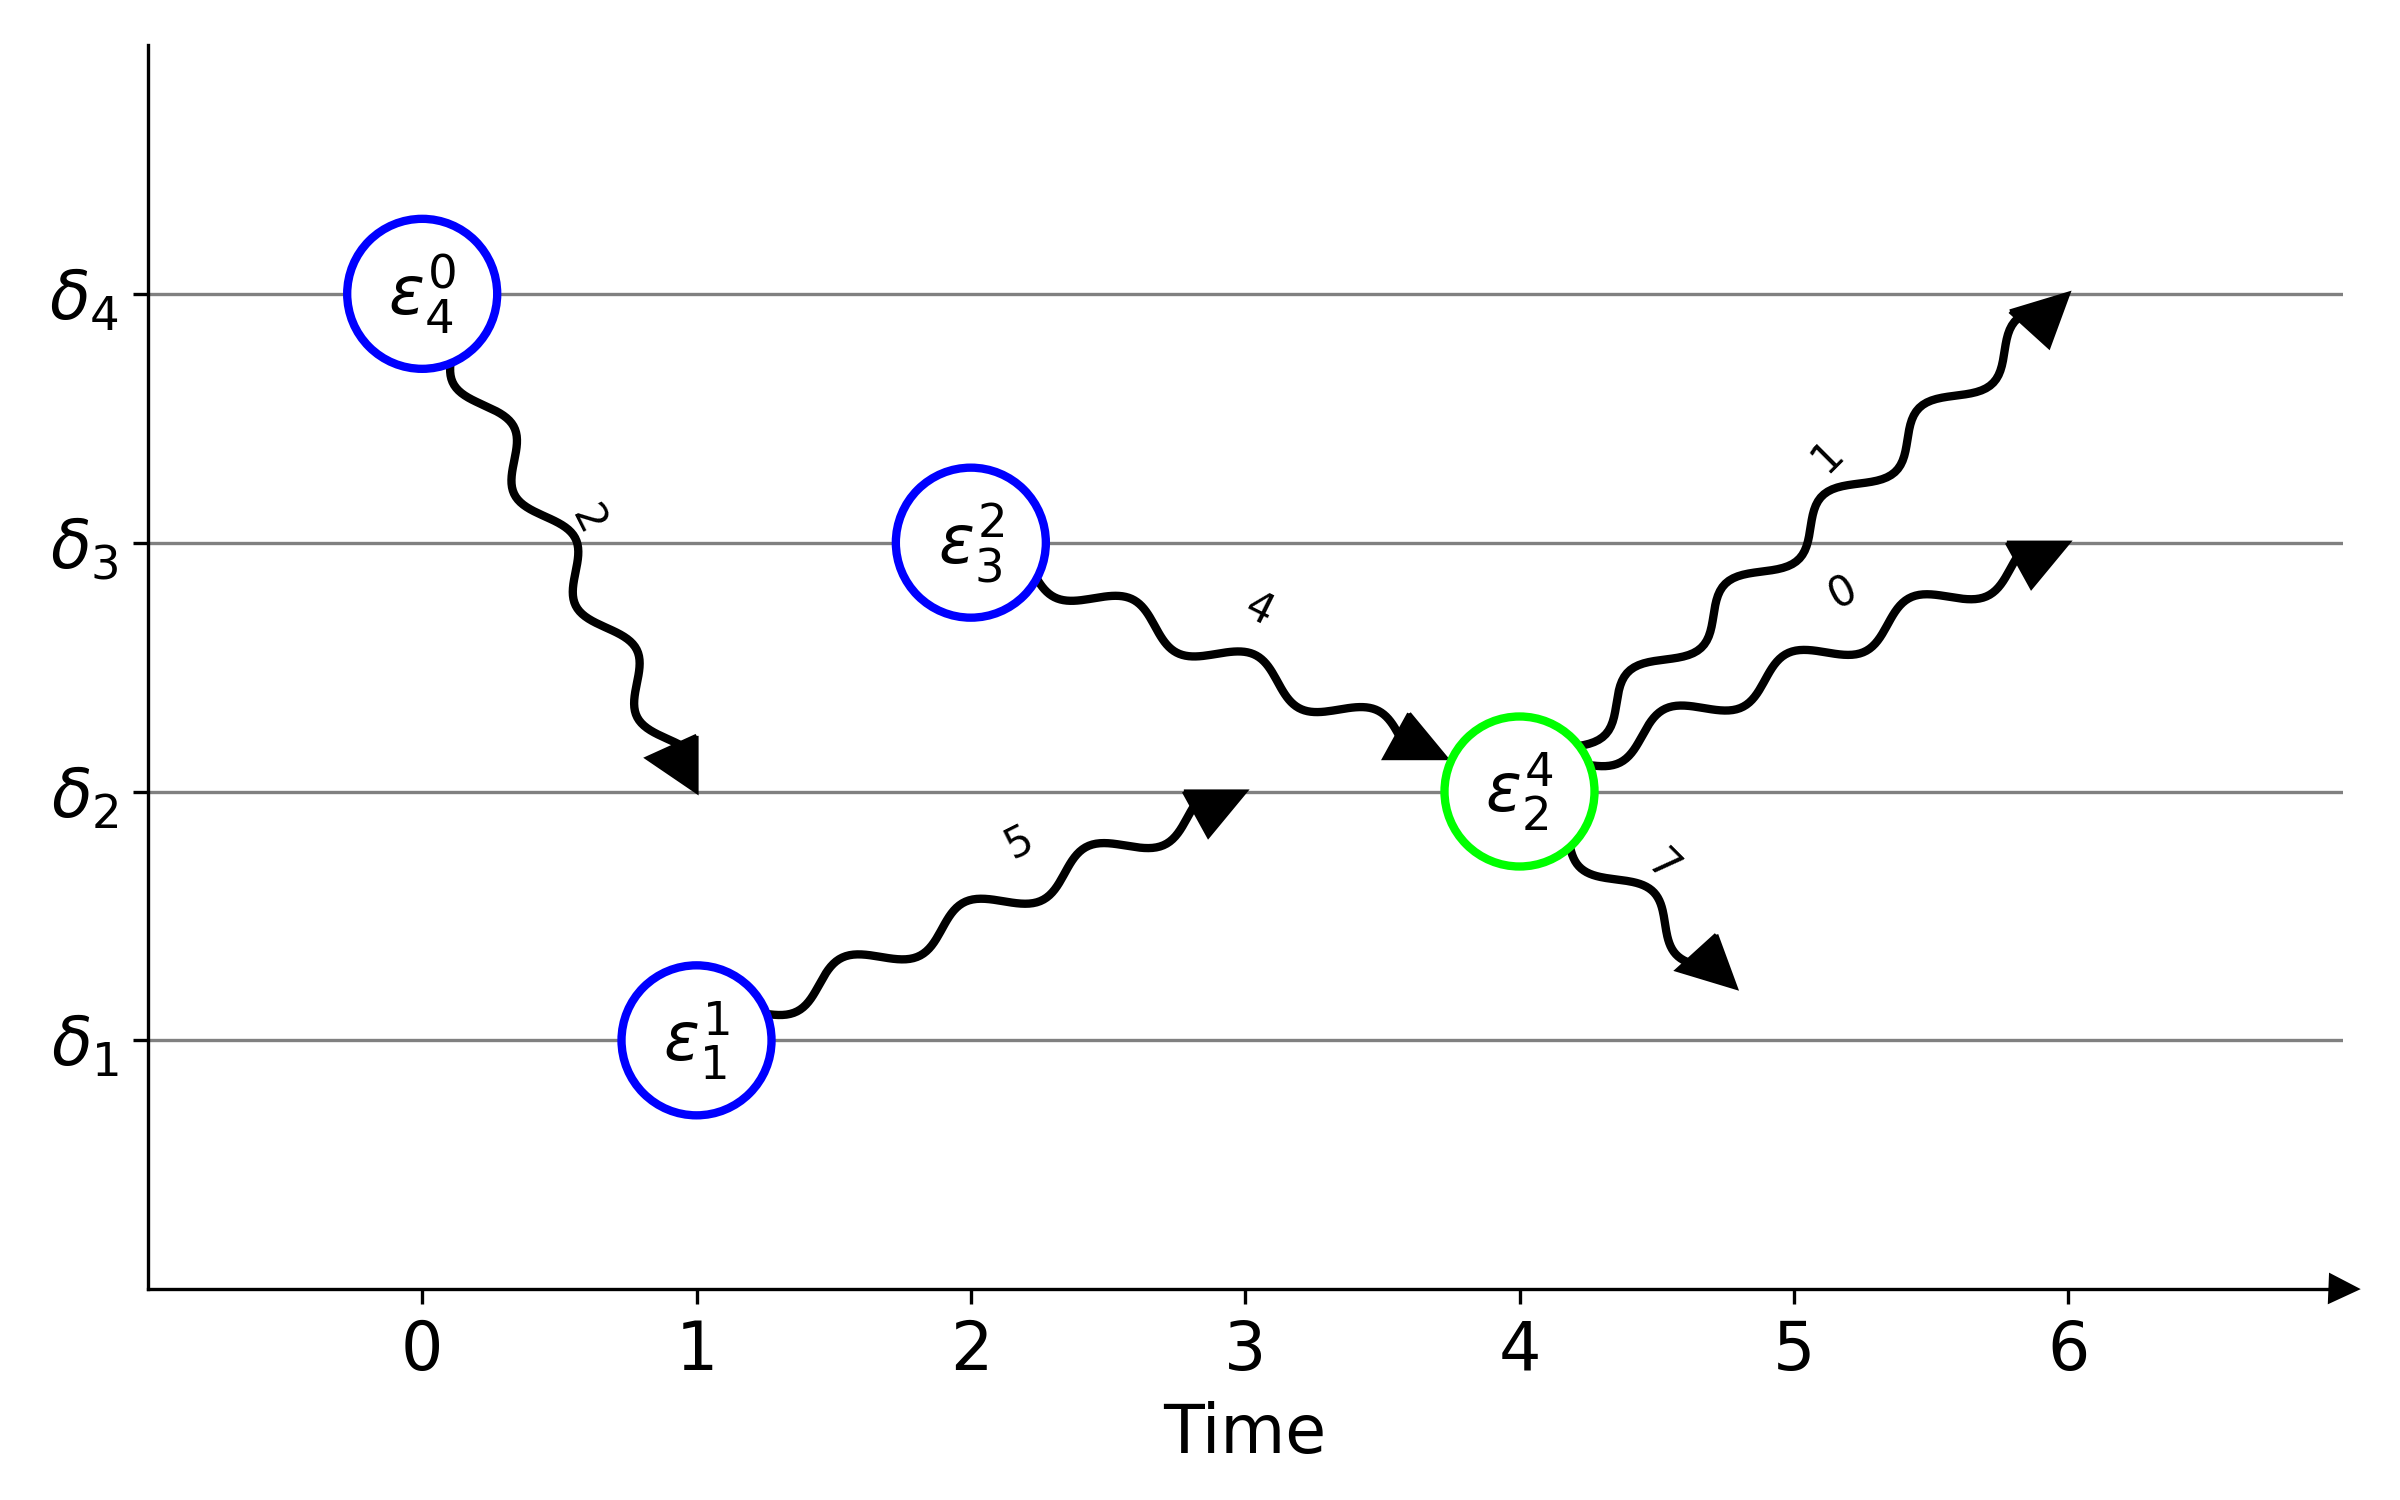
\includegraphics[width=.8\linewidth]{figures/nvalues-example.png}
    \caption{XC system model, from the point of view of the wake-up event $\epsilon_2^4$ pictured in green.}
    \label{fig:xc-nvalues-exampke}
\end{figure}

\paragraph{Additional built-in operations} on nvalues are $self(\underline{\mathbf{w}} : \underline{A}) : A$ which returns the local value $\underline{\mathbf{w}}(\delta)$ for the self device $\delta$, and $updateSelf(\underline{\mathbf{w}} : \underline{A}, l : A) : \underline{A}$ which returns a new nvalue with the same content of $\underline{\mathbf{w}}$ but with the value for the self device replaced by $l$~\cite{xc}.
%
Given the built-in function $uid$ that returns the device identifier of the self device, the following property holds: $self(\underline{\mathbf{w}}) = \underline{\mathbf{w}}(uid)$.
%
The complete syntax for \ac{XC} is available in the original paper~\cite[p. 4]{xc}.

\subsection{The \quotes{exchange} primitive}

The following description is based on the original paper for \ac{XC}~\cite{xc}.
%
The only communication primitive present in \ac{XC} is the function $$exchange(e_i, (\underline{\mathbf{n}}) \Rightarrow \mathbf{\return} e_r \mathbf{\send} e_s)$$ which is defined using syntactic sugar and translates to $$exchange(e_i, (\underline{\mathbf{n}}) \Rightarrow (e_r, e_s))$$
%
The evaluation of the primitive follows three steps:
\begin{enumerate}
    \item the device evaluates the expression $e_i$ to obtain the \textit{initial} local value $l_i$;
    \item $\underline{\mathbf{n}}$ is substituted with the nvalue $\underline{\mathbf{w}}$ of messages received from neighbors for this exchange, using $l_i$ as the default value for $\underline{\mathbf{w}}$, and the device evaluates the expression $e_r$ to the value $v_r$ to be returned;
    \item the device evaluates the expression $e_s$ to obtain a nvalue $\underline{\mathbf{w_s}}$ to be sent to neighbors such as $\delta'$, that will use their corresponding value $\underline{\mathbf{w_s}}(\delta')$ in their next execution round.
\end{enumerate}

As a shorthand, $$exchange(e_i, (\underline{\mathbf{n}}) \Rightarrow \mathbf{\return} e \mathbf{\send} e)$$ can be written as $$exchange(e_i, (\underline{\mathbf{n}}) \Rightarrow \mathbf{\retsend} e)$$ according to the \ac{XC} paper~\cite{xc}.

Two examples of reusable functions written in \ac{XC} can be seen in \Cref{lst:xc-program}.
%
There, $mux(cond, e_1, e_2)$ is a conditional expression that first evaluates $cond$, $e_1$, and $e_2$, and then returns the value of $e_1$ if $cond$ is true, or the value of $e_2$ otherwise.
%
\texttt{mux} is useful to avoid breaking the alignment of the network by using conditionals, as explained in \Cref{chap:background->sec:xc->subsec:alignment}.
%
In the examples provided, $\underline{senseDist}$ is a network-based sensor that returns the nvalue containing the distances to neighbors, abstracting over the way the device obtains the measurements, with $Infinity$ as its default value used for all other devices.
%
\texttt{distanceEstimate} computes the minimum distance from a source using the distance sensor and the neighbors estimate $\underline{\mathbf{n}}$ of their minimum distance from the same source.
%
\texttt{distanceTo} computes the minimum distance from a source determined by a boolean expression $src$, which is represented as a \textit{gradient} with value:
\begin{itemize}
    \item $0$ in all the devices where $src$ is true;
    \item the distance from the closest source in all the devices where $src$ is false that are connected to at least one source;
    \item $Infinity$ otherwise.
\end{itemize}

\lstinputlisting[float,language=XC,label={lst:xc-program}, caption={Implementation of a network-wide gradient, called \texttt{distanceTo}, using the XC language.}]{listings/xc-gradient-distance.xc}

\subsection{Alignment}\label{chap:background->sec:xc->subsec:alignment}

A program can execute multiple exchanges in a single round and \ac{XC} ensures that messages are dispatched to corresponding exchange expressions using the concept of \textit{alignment}.
%
The corresponding exchange expressions are those that are located in the same position within the \ac{AST} and same stack frame, thus ensuring correct alignment in case of branches, function calls, and recursion~\cite{xc}.
%
As a consequence, the evaluation of an aggregate program implicitly builds a tree representation, called \textit{value tree}.
%
All the aligned devices replicate and then exchange the value tree with each other, including the device itself in the next rounds.

Conditionals such as $if\;(cond)\;{e_1}\;else\;{e_2}$ interfere with alignment because only the \texttt{exchange} operations in the same position within the \ac{AST} and stack frame align~\cite{xc}.
%
As a consequence, \texttt{exchange} only aligns across devices that take the same branch of all the conditionals that are the parent or the ancestor of the \texttt{exchange} operation in the \ac{AST}.

Alignment controls the evaluation of sub-expressions, in particular the evaluation of expressions involving nvalues, because in such expressions only aligned neighbors are considered.
%
As a result, every \texttt{if} expression splits the network into two non-communicating sub-networks, with each device evaluating a different branch based on the condition~\cite{xc}.
%
These isolated sub-networks are also referred to as \textit{sub-domains} or simply \textit{domains}.

\subsection{Formalization of XC}

\ac{XC} is formalized in the paper~\cite{xc} in its syntax, operational semantics, and denotational semantics.
%
The language takes inspiration from \ac{ML} and is a standard functional language with a classic Hindley-Milner type system.
%
Its formalization makes \ac{XC} type sound and deterministic once extended with \textit{value-tree} typing and \textit{configuration} typing~\cite{xc}.

\subsection{Implementing FC primitives with exchange}

Since \ac{FC} primitives and expressiveness can be implemented through \ac{XC}, \ac{XC} inherits all the findings reported in the literature that hold for \ac{FC}.
%
These include eventual recovery and stabilization after transient changes~\cite{self-stabilisation-in-fc}, independence from the density of devices~\cite{density-independence-in-fc}, real-time error tolerance, and convergence~\cite{real-time-error-tolerance-in-fc}.
%
Furthermore, the list of benefits extends beyond these~\cite{xc}.
%
Additionally, \ac{XC} opens the possibilities for writing programs not expressible with \ac{FC}, thanks to the expressiveness of the \texttt{exchange} primitive which allows sending differentiated messages to neighbors.
%
In \ac{FC}, the concept of \textit{field}, also called \textit{neighboring value}, is defined as a neighbor-dependent value consisting of a map $\phi = \overline{\delta} \mapsto \overline{l}$ from neighbors to local values, which can be promoted to nvalue with any valid default value $l$.
%
This preserves the behavior of programs written in \ac{FC} but interpreted within \ac{XC}~\cite{xc}.

\ac{FC} presents three main primitives, all implementable through \ac{XC}:
\begin{itemize}
    \item \texttt{nbr}, used to access the neighbors' values~\cite{from-dc-to-fc-and-ap};
    \item \texttt{rep}, used to compute a new value of an expression based on the result of the same expression in the previous round~\cite{from-dc-to-fc-and-ap};
    \item \texttt{share}, used to efficiently access neighbors' values while computing a new value from the previous result with a single primitive~\cite{share-operator}.
\end{itemize}

The \texttt{nbr} primitive can be implemented as: $$nbr(e: A): \underline{A} = exchange(e, (\underline{n}) \Rightarrow \return \underline{n} \send e)$$
%
The \texttt{rep} primitive can be implemented as: $$rep(e_i: A)\{(x) \Rightarrow e_n\}: A = exchange(e_i, (\underline{x}) => \retsend e_n[x := self(\underline{x})])$$
%
The \texttt{share} primitive can be implemented as: $$share(e_i: A)\{(\underline{x}) \Rightarrow e_n\}: A = self(exchange(e_i, (\underline{x}) => \retsend e_n))$$

\section{Scala 3}\label{chap:background->sec:scala3}

Scala is a statically typed, general-purpose programming language designed to express common programming patterns in a concise, elegant, and type-safe way.
%
Scala 3 is the latest major release of the Scala language, a high-level programming language that combines object-oriented and functional programming paradigms.
%
It is compiled using the \textit{Dotty} compiler\footnote{\url{https://github.com/lampepfl/dotty}}, which is based on the \ac{DOT} calculus~\cite{dot}, while Scala 2 is compiled using the \textit{scalac} compiler\footnote{\url{https://github.com/scala/scala}}.
%
This section provides an overview of the main features of Scala 3, that are relevant for the re-design of ScaFi while also highlighting the differences between Scala 2 and Scala 3.

\subsection{General considerations on Scala 3}

Even though Scala 3 introduces breaking changes in the syntax from Scala 2, most of the code written in Scala 2 can be compiled with Dotty and is also binary compatible with Scala 2.
%
The Scala community has exploited this possibility to avoid reimplementing a new standard library for Scala 3, using the Scala 2 standard library instead, rewritten to be cross-compiled for both Scala 2 and Scala 3.

Natively, Scala 2 and Scala 3 compile to \ac{JVM} bytecode, but Scala 3 also supports the \ac{JS} and \textit{LLVM} backends, which are used to compile Scala code to JavaScript and native code, respectively.
%
These compiler backends exist thanks to community-driven projects\footnote{Scala.js at \url{https://scala-js.org}}\footnote{Scala Native at \url{https://scala-native.org}}~\cite{scala-js}.
%
The provided support for cross-platform distribution, together with the popularity of Scala for distributed systems development~\cite{scala-popularity} and the flexibility of the upgraded language features for advanced internal \ac{DSL} design, makes Scala 3 a valuable choice for a new ScaFi implementation based on \ac{XC}.

\subsection{Values in Scala}

In Scala, every value has a type, which follows the type hierarchy explained in \Cref{chap:background->sec:scala3->subsec:type-hierarchy}.
%
When declaring a new variable or field as a container of a value, the type can either be explicitly declared or inferred by the compiler.
%
Every declaration of a variable or field must be preceded by the \texttt{val} keyword for an immutable value or the \texttt{var} keyword for a mutable value.
%
Immutable values cannot be reassigned, while mutable values can be reassigned, but their type cannot be changed.
%
It is worth noting that \texttt{val} does not guarantee that the value itself is immutable, but only that the reference to the value cannot be changed.


\subsection{New control syntax and significant indentation}

Scala 3 introduces a new syntax for control expressions, as well as new rules that allow the indentation alone to replace the use of curly braces.
%
Both these changes are aimed at making the code more readable and concise, sometimes noticeably closer to the natural language.
%
For instance, in \Cref{lst:scala2-with-braces}, the \texttt{if} expression is written with the traditional syntax, while in \Cref{lst:scala3-without-braces} the same expression is written using the new syntax.
%
The same is true for the \texttt{for} expression, the \texttt{while} loop, and the \texttt{match} expression.

\lstinputlisting[float,language=Scala,label={lst:scala2-with-braces}, caption={Examples of syntax using braces in Scala 2.}]{listings/scala2-with-braces.scala}
\lstinputlisting[float,language=Scala,label={lst:scala3-without-braces}, caption={Examples of syntax avoiding braces in Scala 3.}]{listings/scala3-without-braces.scala}

In cases where a code block consists of many lines that make it difficult to follow the indentation, the new syntax can be augmented with \texttt{end} statements, as demonstrated in \Cref{lst:scala3-with-end}.

\lstinputlisting[float,language=Scala,label={lst:scala3-with-end}, caption={Example of syntax using \texttt{end} statements in Scala 3.}]{listings/scala3-without-braces-with-end.scala}


\subsection{Traits and classes}

Traits are a powerful feature that replaces Java's interfaces and abstract classes and were first introduced as a mechanism to organize behavior into small, modular units~\cite{traits}.
%
In Scala, traits can be used to define interfaces and to provide partial implementations and can be composed and mixed into other traits or classes.
%
With Scala 3, traits are now able to have parameters like classes do, enhancing their expressiveness.
%
Furthermore, Scala 3 introduces new rules for the instantiation of classes that enable the avoidance of the \texttt{new} keyword, as shown in \Cref{lst:scala3-without-braces}.
%
This feature is called \textit{universal apply methods} and is implemented by the generation of \texttt{apply} methods for classes when the user does not provide one, during the compilation.
%
Another enabling factor is the special role given to methods named \texttt{apply}, which in Scala can be invoked without the need to specify the method name.
%
When combined with companion objects, described in \Cref{chap:background->sec:scala3->subsec:singleton-objects}, it is often possible to replace auxiliary constructors in classes with multiple \texttt{apply} methods in the companion object, which is a typical pattern in Scala.
%
Anonymous classes can also be used to instantiate a trait or abstract class by providing a concrete implementation of abstract methods on the fly.
%
In addition, traits, classes, and singleton objects can be nested, and they can access each other's private members, just like in Java.

If the definition of something depends on another from a different package, it is possible to use the \texttt{import} keyword to import the needed definitions.
%
\texttt{import} statements can be put at the beginning of a file or inside a block and can be used to import a single definition, a group of definitions, or all definitions from a package.
%
Additionally, Scala supports import aliases to avoid name clashes.
%
Since Scala 3, import aliases have a dedicated syntax, following the pattern \texttt{import A as B}, where \texttt{A} is the fully qualified original name and \texttt{B} is the alias.

An advanced example of trait usage can be found in \Cref{lst:scala3-service-oriented-design}\footnote{\url{https://docs.scala-lang.org/scala3/book/domain-modeling-oop.html}}, which shows how to use traits in a service-oriented way, a design pattern that promotes the use of traits to define services and their dependencies and to compose services into a single class~\cite{service-oriented-design}.
%
In the mentioned example, some advanced features of Scala are presented, such as abstract type members, nested traits, and \textit{self-type annotations}.
%
The \textit{self-type annotation} is a way to declare that a trait must be mixed into a class that extends another trait, and it is used to express dependencies between traits without resorting to inheritance.
%
Self-type annotations allow the composition of traits to be more flexible and less coupled and delay the choice of trait order of linearization to the class that mixes them.

\lstinputlisting[float,language=Scala,label={lst:scala3-service-oriented-design}, caption={Advanced example of usage of traits, know as service-oriented design. The code was taken from the Scala 3 book.}]{listings/scala3-service-oriented-design.scala}

\subsubsection{Object-oriented programming in Scala 3}

In Scala, methods for classes, traits, enums, and objects can be defined using the \texttt{def} keyword, as shown in \Cref{lst:scala3-without-braces}.
%
Abstract methods do not have a body and must be overridden by concrete subclasses, while concrete methods have a body and can be overridden by subclasses.
%
Moreover, Scala allows a method with no arguments to be overridden by a field with the same name.
%
Additionally, methods can serve as operators using infix notation, enabling invocation with a single argument without using the dot or parentheses, as demonstrated in \Cref{lst:exchange-syntax}.
%
This feature provides flexibility in defining custom operators and developing \ac{DSL}s.
%
Since Scala 3, the \texttt{infix} keyword must precede \texttt{def} to explicitly denote the intent of defining custom operators.

Even though method overloading is still possible, the Java generic type erasure rules apply in Scala too, and must be taken into account when defining overloaded methods.
%
In Scala, it is often possible to avoid method overloading by using default arguments, which are arguments that are automatically assigned a value if no value is provided by the caller, as shown in \Cref{lst:scala3-extension-methods}.
%
Scala 3 improves the default way to handle most method invocation ambiguities with the \texttt{@targetName} annotation, allowing the specification of a unique name for the method once compiled to \ac{JVM} bytecode.

Thanks to \textit{automatic eta expansion}, methods can be used in place of function values, and its implementation has been improved in Scala 3 to be almost completely seamless.

One of the most important features of Scala is the ability to define \textit{type members},
which are members of a class or trait that define types, and can be used as types in the same way as classes or traits, as shown in \Cref{chap:background->sec:scala3->subsec:type-system}.
%
Abstract type members prevent Scala traits' and classes' sources from growing in size both vertically and horizontally, as they can often replace generic type parameters with all the benefits of member inheritance, such as overriding and composition.
%
Type parameters, as well as type members, can be constrained with \textit{upper bounds} and \textit{lower bounds}, using the operators \texttt{<:} and \texttt{>:}, respectively, such as in \texttt{Type <: Supertype} and \texttt{Type >: Subtype}.
%
Additionally, generic types also support type variance control, which is used to specify how the subtyping relationship between two generic types is related to the subtyping relationship between their type arguments as explained in depth in the dedicated section below.

\subsection{Algebraic Data Types}

The union of the object-oriented and the functional programming paradigms within Scala has promoted the use of algebraic data types, a kind of composite type that resembles mathematical operations between types.
%
Examples of such types are \textit{sum types}, \textit{product types}, and \textit{intersection types}.
%
In Scala 2 these can be implemented using \textit{sealed traits}, \textit{case classes}, and inheritance, respectively.
%
However, since Scala 3, the syntax for defining these types has been simplified and clarified, as elaborated in the following paragraphs.

\subsubsection{Sum types}

Since Scala 2, sum types were enabled by the \texttt{sealed} modifier on traits or abstract classes, which prevents inheritance outside the file where the sum type is defined.
%
This way, it is possible to define a finite set of subtypes to check for in pattern matching.
%
Moreover, the ability to define a singleton instance with the \texttt{object} keyword inheriting from the sum type enables the use of sum types for implementing enumerations.
%
With the introduction of Scala 3, the \texttt{enum} keyword simplifies the syntax in both the mentioned use cases, as shown in \Cref{lst:scala3-sum-types}.
%
Additionally, with Scala 3, the \texttt{|} operator can be used for sum type options in type definitions, for matching any pattern of a list in pattern matching, and for defining discriminated union types of the form \texttt{A | B}.

\lstinputlisting[float,language=Scala,label={lst:scala3-sum-types}, caption={Example of sum types in Scala 3.}]{listings/scala3-enums.scala}

\subsubsection{Product types}

Product types, supported since Scala 2, are enabled by the features provided by \textit{case classes}, which are Scala's implementation of the concept of \textit{records} in functional programming.
%
Case classes are equipped with compiler-generated methods for pattern matching, equality, copying, and printing.
%
In case classes, constructor parameters are public immutable fields by default, and the \texttt{copy} method can be used to create a new instance with specified fields altered.
%
An example of a case class can be found in \Cref{lst:scala3-sum-types}.

\subsubsection{Intersection types}

Since Scala 2, it is possible to define a type as the intersection of other types using the \texttt{with} keyword, which is also used for mixin composition.
%
Mixin composition is the practice of combining multiple traits into a class, resembling multiple inheritance, but with the compromise of avoiding the diamond problem through linearization~\cite{scala-patterns}.
%
Mixin composition is employed in ScaFi to declare dependencies of programs, as shown in \Cref{lst:using-libraries-in-scafi}.

Starting with Scala 3, the \texttt{with} keyword is deprecated for type definitions, such as in method arguments, in favor of the \texttt{\&} operator.
%
This operator is also used for pattern matching, as in \Cref{lst:distance-to}, within the \texttt{distanceTo} signature.
%
Although deprecated for type definitions, the \texttt{with} keyword is still used for mixin composition in the definition of traits and classes.


\subsection{Singleton objects} \label{chap:background->sec:scala3->subsec:singleton-objects}

In Scala, the \texttt{object} keyword is used to define singleton objects which are classes with only one instance.
%
Singleton objects serve as a replacement for Java's static methods and fields and can be used to define utility methods and constants, as well as to implement the \textit{companion object} pattern.
%
This pattern promotes the use of a singleton object to hold methods and fields that are not specific to any instance of a class but are still related to the class itself.
%
A class with a companion object can access the private members of the companion object, and vice versa, provided that they share the same name and are defined in the same file.
%
Moreover, singleton objects can be used to implement traits to create \textit{modules}, such as factories for collections.
%
An example of a singleton object used as a companion of a class can be found in \Cref{lst:scala3-singleton-object}.

\lstinputlisting[float,language=Scala,label={lst:scala3-singleton-object}, caption={Example of a singleton object in Scala 3.}]{listings/scala3-singleton-object.scala}


\subsection{Functional programming with Scala 3} \label{chap:background->sec:scala3->subsec:functional-programming}

Scala offers many features typical of \ac{FP} languages, including \textit{lambdas}, higher-order functions (i.e., functions that accept or return other functions), \textit{currying}, algebraic data types, and a standard library of immutable collections.
%
Lambdas, also known as anonymous functions, can be treated as any other value, thus passed as arguments, or returned as results.
%
In Scala, lambdas are defined using the \texttt{=>} operator, which is also used for defining function types such as \texttt{A => B}, where \texttt{A} denotes the input type and \texttt{B} denotes the output type.
%
In some cases, it is possible to write lambdas with a more concise syntax, using the \texttt{\_} placeholder for the input argument, as shown in \Cref{lst:foldhood-library-usage}.

Scala 3 introduces new varieties of function types:
\begin{itemize}
    \item \textit{dependent function types}, where the result type can depend on the function's parameters, such as type members (an example can be found in \Cref{lst:distance-to});
    \item \textit{polymorphic function types}, that accept type parameters, explained in \Cref{chap:background->sec:scala3->subsec:type-system};
    \item \textit{context function types}, that accept only context parameters, explained in \Cref{chap:background->sec:scala3->subsec:contextual-abstractions}.
\end{itemize}

Following the principles of \ac{FP}, domain models should be immutable and deprived of behavior.
%
More specifically, the behavior should be defined in terms of pure functions implemented in modules as extension methods, which are methods that can be added to existing types without modifying their source code.
%
Starting with Scala 3, extension methods have obtained a dedicated syntax that avoids the cumbersome use of implicit classes, as shown in \Cref{lst:scala3-extension-methods}.
%
However, some additional attention is needed when extension method names overlap with class methods, as the compiler prioritizes class methods, potentially shadowing conflicting extension methods.
%
In such cases, it may be necessary to invoke the extension explicitly from the instance that provides it, passing the extended instance as the first argument.

\lstinputlisting[float,language=Scala,label={lst:scala3-extension-methods}, caption={Example of extension methods usage in Scala 3.}]{listings/scala3-extension-methods.scala}

\paragraph{Currying} is the process of transforming a function that accepts multiple arguments into a sequence of functions, each taking a subset of the arguments, thus simplifying the function's usage with partial applications.
%
An example of currying and partial application of a function is present in \Cref{lst:scala3-currying}.

\lstinputlisting[float,language=Scala,label={lst:scala3-currying}, caption={Example of currying and partial application in Scala 3.}]{listings/scala3-currying.scala}


\subsection{Contextual Abstractions} \label{chap:background->sec:scala3->subsec:contextual-abstractions}

In Scala, contextual abstractions derive from the core concept of \textit{term inference}, which is the ability of the compiler to synthesize a \quotes{canonical} term for a given type.
%
Examples of features enabled by term inference are \textit{extension methods}, \textit{type classes}, \textit{context parameters}, and \textit{context bounds}.
%
While in Scala 2 almost every feature related to contextual abstractions was enabled by the \texttt{implicit} keyword, Scala 3 contextual abstractions have been redesigned to be more explicit on the intent of their usage, with the introduction of new ad-hoc keywords for each use case: \texttt{given}, \texttt{using}, and \texttt{extension}.
%
The \texttt{given} keyword is used to define a \textit{given instance}, which is a value to be passed as a \textit{context parameter} in methods or constructors that require one.
%
The \texttt{using} keyword defines such \textit{context parameters}, which are method parameters requiring a \textit{given instance} available in scope and correspond to implicit parameters of Scala 2.
%
If given instances are not passed explicitly as context parameters, the compiler performs \textit{term inference} to search for \textit{given instances} in scope to fulfill \textit{context parameters} at every method invocation.
%
Starting with Scala 3, context parameters can be anonymous, and given instances can be abstract.
%
The \texttt{extension} keyword is now necessary to define \textit{extension methods}, enabling the addition of methods to existing types without altering their source code, as explained in \Cref{chap:background->sec:scala3->subsec:functional-programming}.
%
To retrieve the value of an anonymous context parameter of type \texttt{T} Scala 3 provides the \texttt{summon[T]: T} method, replacing Scala 2's \texttt{implicitly[T]} method.

\textit{Context bounds} in the form \texttt{T: Type} are syntactic sugar for context parameters with a more concise syntax, that gets desugared by the compiler to a context parameter of type \texttt{Type[T]}.
%
For example, in \Cref{lst:distance-to}, \texttt{N:Numeric:UpperBounded} is desugared to two new context parameters in the form \texttt{(using Numeric[N], UpperBounded[N])}.
%
An abstract class like \texttt{Type[T]} designed to add behavior to any closed data type without sub-typing is called a \textit{type class}.

Given instances can be imported and exported using the \texttt{import} and \texttt{export} keywords.
%
However, in Scala 3, \textit{given imports} and \textit{given exports} require the \texttt{given} keyword, even where a wildcard is used, enhancing clarity regarding their origin within the current scope.
%
Moreover, Scala 3 allows for anonymous concrete given instances, for which the compiler synthesizes a name automatically.
%
This feature is useful to avoid polluting the namespace with names that are not meant to be used directly by the user, because often given instances are imported by their type instead of by their name.

Starting with Scala 3, implicit conversions are defined by providing given instances of the type \texttt{Conversion[From, To]} and must be enabled with a compiler flag to prevent warnings when conversion is silently applied before passing an argument to a function call.
%
By default, the Scala compiler provides implicit conversions for primitive types, such as \texttt{Int} to \texttt{Long}.


\subsection{The Scala 3 type system} \label{chap:background->sec:scala3->subsec:type-system}

Scala, being a statically typed language, has all the benefits of early error detection, better performance, and robust tooling support.
%
However, it also provides a flexible environment typical of dynamically typed languages, thanks to features like type inference, type parameters, and type members.
%
Built upon a variant of the Hindley-Milner type system, Scala's type inference system supports subtyping, generics, and type bounds, as Java does.
%
Additionally, Scala offers many type system features absent in Java, such as \textit{type variance}, \textit{type aliases}, \textit{type members}, \textit{covariant and contravariant overriding}, \textit{higher-kinded types}
%
Furthermore, starting with Scala 3, the type system features \textit{opaque type aliases}, \textit{structural types}, \textit{dependent function types}, improved \textit{type lambdas}, \textit{polymorphic function types}, \textit{context function types}, and \textit{match types}.
%
In the following paragraphs, the most relevant features of the Scala 3 type system are explained.

\paragraph{Type variance} allows specifying how the subtyping relationship between two generic types is related to the subtyping relationship between their type arguments.
%
In Scala, the variance of a type parameter can be declared with the \texttt{+} and \texttt{-} symbols, which are used to declare a type parameter as covariant or contravariant, respectively, else the type parameter is invariant by default.
%
A usage example of a variant annotation is present in \Cref{lst:scala3-sum-types}.

\paragraph{Type aliases} are used to define new names for existing types, which are often more descriptive or shorter than the original names.
%
Type aliases can be parameterized and can be recursive.
%
Their syntax is the same for defining type members, using the \texttt{type} keyword, as shown in \Cref{lst:scala3-opaque-type-alias}.
%
Opaque type aliases are a new feature of Scala 3 that allows defining a type alias that is not interchangeable with its underlying type, hiding it from consumers.

\lstinputlisting[float,language=Scala,label={lst:scala3-opaque-type-alias}, caption={Example of opaque type alias and covariant override in Scala 3.}]{listings/scala3-opaque-type-alias.scala}

\paragraph{Covariant overrides} enable the overriding of superclass methods with methods that have more specific return types, as shown in \Cref{lst:scala3-opaque-type-alias}.

\paragraph{Higher-kinded types} allow the definition of types and methods that work on generic types regardless of their actual type arguments, only requiring a fixed arity of type parameters.
%
Scala types are partitioned into kinds based on the top type of which it is a subtype, such as \texttt{Any}, \texttt{[+X] =>> Any}, \texttt{[X, +Y] =>> Any}.
%
Higher-kinded types have a kind that counts at least one type arrow, such as \texttt{List} of kind \texttt{[+X] =>> Any}, \texttt{Option} of kind \texttt{[+X] =>> Any}, and \texttt{Map} of kind \texttt{[X, +Y] =>> Any}, but potentially even a type whose kind is \texttt{[X] =>> [Y] =>> Any}, such as a type class for a type constructor.
%
Scala 3 adds support for \textit{kind polymorphism}, allowing the definition of type parameters that accept types of any kind, through the special syntax \texttt{T <: AnyKind}.

\paragraph{Type lambdas} are simply anonymous type constructors, that starting from Scala 3 have a new concise syntax thanks to the type operator \texttt{=>>}.
%
For instance, \texttt{[X, Y] =>> Map[Y, X]} is a binary type constructor that maps arguments \texttt{X} and \texttt{Y} to the type \texttt{Map[Y, X]}.

\paragraph{Context functions} are functions that accept only context parameters as input.
%
Starting with Scala 3, context functions can be treated as values thanks to context function types, which can be distinguished from standard function types by the presence of the \texttt{?=>} operator in place of the \texttt{=>} operator.

\paragraph{Match types} are conditional type aliases that allow the definition of a type as the result of a pattern match between types, and are available only in Scala 3.
%
An example of match types can be found in \Cref{lst:scala3-match-types}.

\lstinputlisting[float,language=Scala,label={lst:scala3-match-types}, caption={Example of match types in Scala 3.}]{listings/scala3-match-type.scala}


\subsection{Explicit nulls and the Scala 3 type hierarchy} \label{chap:background->sec:scala3->subsec:type-hierarchy} \label{chap:background->sec:scala3->subsec:explicit-nulls}

The Dotty compiler offers experimental features that alter the language in various ways.
%
Two examples of experimental features relevant to \this are \textit{explicit nulls} and \textit{multiversal equality}.
%
Explicit nulls are enabled by the \quotes{\texttt{-Yexplicit-nulls}} flag, which modifies the type hierarchy of Scala making reference types non-nullable.
%
With explicit nulls disabled, the type system looks like the one in Java, pictured in \Cref{fig:scala-hierarchy-with-explicit-nulls-disabled}.
%
Conversely, with explicit nulls enabled, the type system resembles Kotlin's, where null safety is a key part of the language, as depicted in \Cref{fig:scala-hierarchy-with-explicit-nulls-enabled}.
%
Nullable values with that option enabled can still be defined using sum types, such as in \texttt{Type | Null}.
%
Scala 3 provides the extension method \texttt{.nn} to convert a nullable value to a non-nullable one through casting.
%
If the value was \texttt{null} at runtime, this forced conversion results in a \textit{NullPointerException}.

\begin{figure}
    \centering
    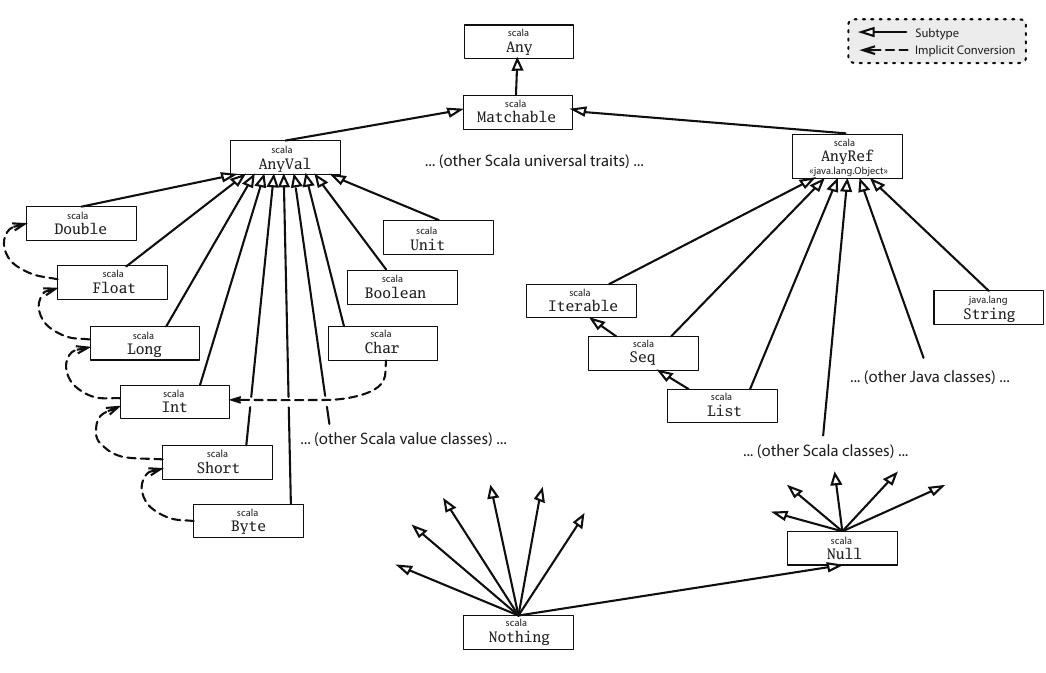
\includegraphics[width=.8\linewidth]{figures/scalaHierarchyWithMatchable.png}
    \caption{Scala type hierarchy with explicit nulls disabled.}
    \label{fig:scala-hierarchy-with-explicit-nulls-disabled}
\end{figure}

\begin{figure}
    \centering
    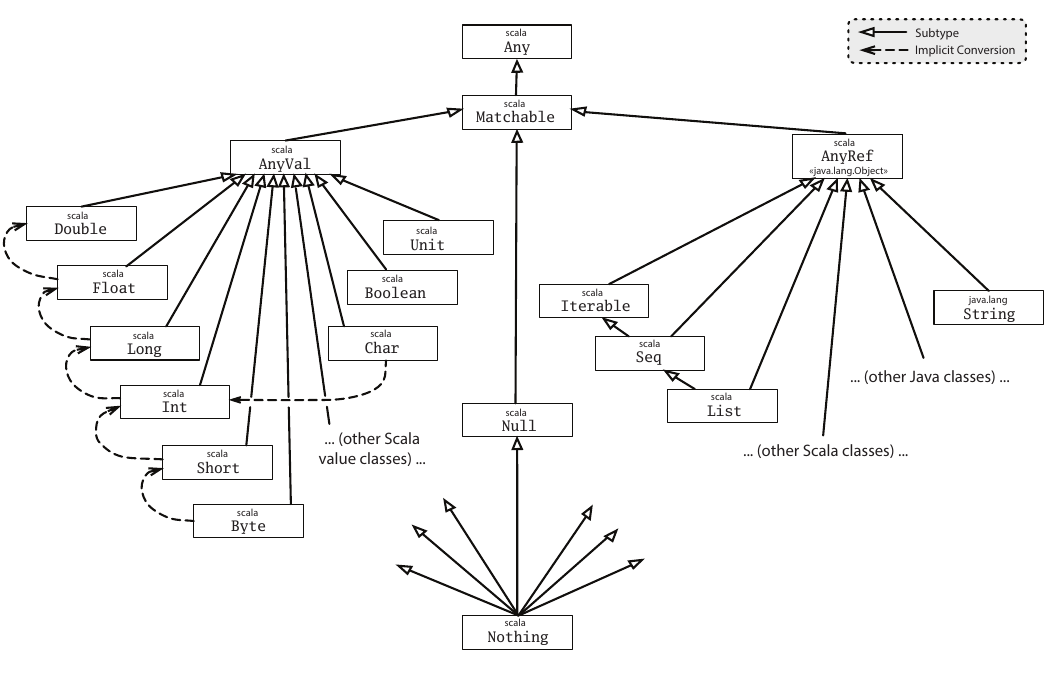
\includegraphics[width=.8\linewidth]{figures/scalaHierarchyWithMatchableAndSafeNull.png}
    \caption{Scala type hierarchy with explicit nulls enabled.}
    \label{fig:scala-hierarchy-with-explicit-nulls-enabled}
\end{figure}


\subsection{Multiversal Equality} \label{chap:background->sec:scala3->subsec:multiversal-equality}

The Scala 3 compiler with the \quotes{\texttt{-language:strictEquality}} flag enabled forbids \textit{universal equality}, that allowed comparing any two values regardless of their types using the \texttt{==} operator, which under the hood invoked the \texttt{equals} method.
%
With that flag enabled, universal equality is replaced with \textit{multiversal equality}, which allows comparing two values of type \texttt{X} and \texttt{Y} only if a given instance of \texttt{CanEqual[X, Y]} can be found.
%
Implementing \texttt{CanEqual[X, Y]} instances can be automated with \textit{type class derivation}, a feature of Scala 3 that allows the compiler to synthesize given instances following rules defined by the user, often based on compositions of algebraic data types.


% ! TeX root = ../thesis-main.tex
%----------------------------------------------------------------------------------------
\chapter{Analysis}
\label{chap:analysis}
%----------------------------------------------------------------------------------------
This chapter defines the scope, requirements, and use cases of \this, based on the expectations of the stakeholders, consisting of ScaFi developers and researchers.
%
A priority analysis is conducted using the MoSCoW method, ensuring that the work stays focused on delivering key features while meeting technical constraints and user preferences.

\section{Requirements analysis} \label{chap:analysis->sec:requirement-analysis}

Since the very beginning, \this aimed to redesign ScaFi using Scala 3 to improve the quality of the code, including but not limited to readability, maintainability, and reusability.
%
This time, the implementation is based on \ac{XC} as the theoretical foundation, through which the \ac{FC} constructs could be implemented.

The project started interviewing the stakeholders, including developers and researchers who developed the original ScaFi and still use it, in order to understand their needs and expectations.

The \textit{key users} identified for the library are:
\begin{itemize}
    \item \textit{End users}, that are the developers who will use the library to implement their aggregate programs;
    \item \textit{Library developers}, who will extend the library with new features, constructs, and syntax;
    \item \textit{Researchers}, who will experiment with the calculus foundations and could benefit from reusing existing libraries.
\end{itemize}

During the stakeholder interviews, a comprehensive list of functional and technical requirements emerged, which were then carefully curated and prioritized through extensive discussions and feedback sessions.

\paragraph{Functional requirements} are the features that the library must provide to the users. The following are the most relevant functional requirements identified:
\begin{enumerate}[label=\textbf{F.\arabic*}]
    \item Redesign and implement a new \ac{API} for the \texttt{core} package\cref{chap:analysis->sec:scafi-analysis};
    \item Redesign and implement the \texttt{tests} package with acceptance tests, easy to read and understand, and that can be used as examples;
    \item Use the \ac{XC} as the foundation of the (default) implementation of constructs, while still providing a \ac{FC} based API;
    \item Develop an \textit{Alchemist incarnation}\footnote{\url{https://github.com/AlchemistSimulator/Alchemist}}~\cite{alchemist}, enabling \this programs to run on the well-tested and widely used Alchemist simulator;
    \item Develop a minimal, pure Scala 3 simulator to run tests and examples without the need for external dependencies;
    \item Provide a new API for the \texttt{core} package that allows developers to import arbitrary ScaFi libraries and constructs into their programs without conflicts, in a seamless way;
    \item Prefer keeping the original, abbreviated names for core constructs like \texttt{nbr} and \texttt{rep}, as they are widely adopted and recognized within the community, promoting consistency and familiarity;
    \item Conduct experiments with Scala 3 to explore and achieve new compile time features for ScaFi, to enhance code quality and elevate the overall user experience.
\end{enumerate}

\paragraph{Technical requirements} are the constraints and guidelines that the library must follow to ensure the quality of code and user experience.
\begin{enumerate}[label=\textbf{T.\arabic*}]
    \item Use Scala 3 as the host language to leverage its advanced features and enhancements;
    \item Enable quality options on the Scala 3 compiler such as explicit nulls (\cref{chap:background->sec:scala3->subsec:explicit-nulls}) and multiversal equality (\cref{chap:background->sec:scala3->subsec:multiversal-equality});
    \item Employ \ac{SBT} as build system;
    \item Cross-build the project for \textit{scala-js}\footnote{\url{https://www.scala-js.org}};
    \item Cross-build the project for \textit{scala-native}\footnote{\url{https://scala-native.org}};
    \item Lint the code with \textit{scalafix}\footnote{\url{https://scalacenter.github.io/scalafix}} and/or \textit{scalafmt}\footnote{\url{https://scalameta.org/scalafmt}};
    \item Avoid using third-party libraries for the \texttt{core} package dependencies.
\end{enumerate}

Following the identification of requirements, a comprehensive discussion and prioritization process was undertaken, guided by the \ac{MoSCoW} method.
%
The results are outlined in detail in Table \ref{tab:requirements-prioritization}.

\begin{table}[ht]
\centering
\caption{Requirements prioritization.}
\label{tab:requirements-prioritization}
\begin{tabular}{|>{\hspace{0pt}}m{0.362\linewidth}|>{\hspace{0pt}}m{0.277\linewidth}|>{\hspace{0pt}}m{0.238\linewidth}|} 
    \hline
    \textbf{Requirement} & \textbf{MoSCoW} & \textbf{Priority}  \\ 
    \hline
    F.1          & must   & high      \\ 
    \hline
    F.2          & must   & high      \\ 
    \hline
    F.3          & must   & high      \\ 
    \hline
    F.4          & could  & low       \\ 
    \hline
    F.5          & must   & high      \\ 
    \hline
    F.6          & should & average   \\ 
    \hline
    F.7          & should & average   \\ 
    \hline
    F.8          & won't  & low       \\ 
    \hline
    T.1          & must   & high      \\ 
    \hline
    T.2          & should & high      \\ 
    \hline
    T.3          & must   & high      \\ 
    \hline
    T.4          & could  & low       \\ 
    \hline
    T.5          & could  & low       \\ 
    \hline
    T.6          & should & low       \\ 
    \hline
    T.7          & should & average   \\
    \hline
\end{tabular}
\end{table}

Finally, before starting with the design of the solution, given that the project is a redesign of an existing library, the requirements were compared with the existing ScaFi library to identify the differences and similarities.


\section{ScaFi} \label{chap:analysis->sec:scafi-analysis}

The ScaFi repository\footnote{\url{https://github.com/scafi/scafi}} is organized in modules, as illustrated in \cref{fig:scafi-project-org}.
%
For most of the use cases, only a small subset of the modules should be imported.
%
The \this project primarily focuses on redesigning and implementing the \texttt{core} package, implicitly including \texttt{commons} module, as well as the \texttt{simulator} and \texttt{tests} packages.
%
However, it should be noted that the simulator implementation planned for this project will be a minimal version written in pure Scala 3, as opposed to the existing \texttt{simulator} module, which is a complex and feature-rich suite of tools for simulating aggregate programs in space and time.
%
Porting the remaining modules, which encompass various \ac{GUI} implementations, demos, and integration with \textit{Akka}\footnote{\url{https://akka.io}} for actual deployment of real-world aggregate applications, is out of the scope of \this, and will be addressed in \cref{chap:conclusion-and-future-work}.

\begin{figure}
    \centering
    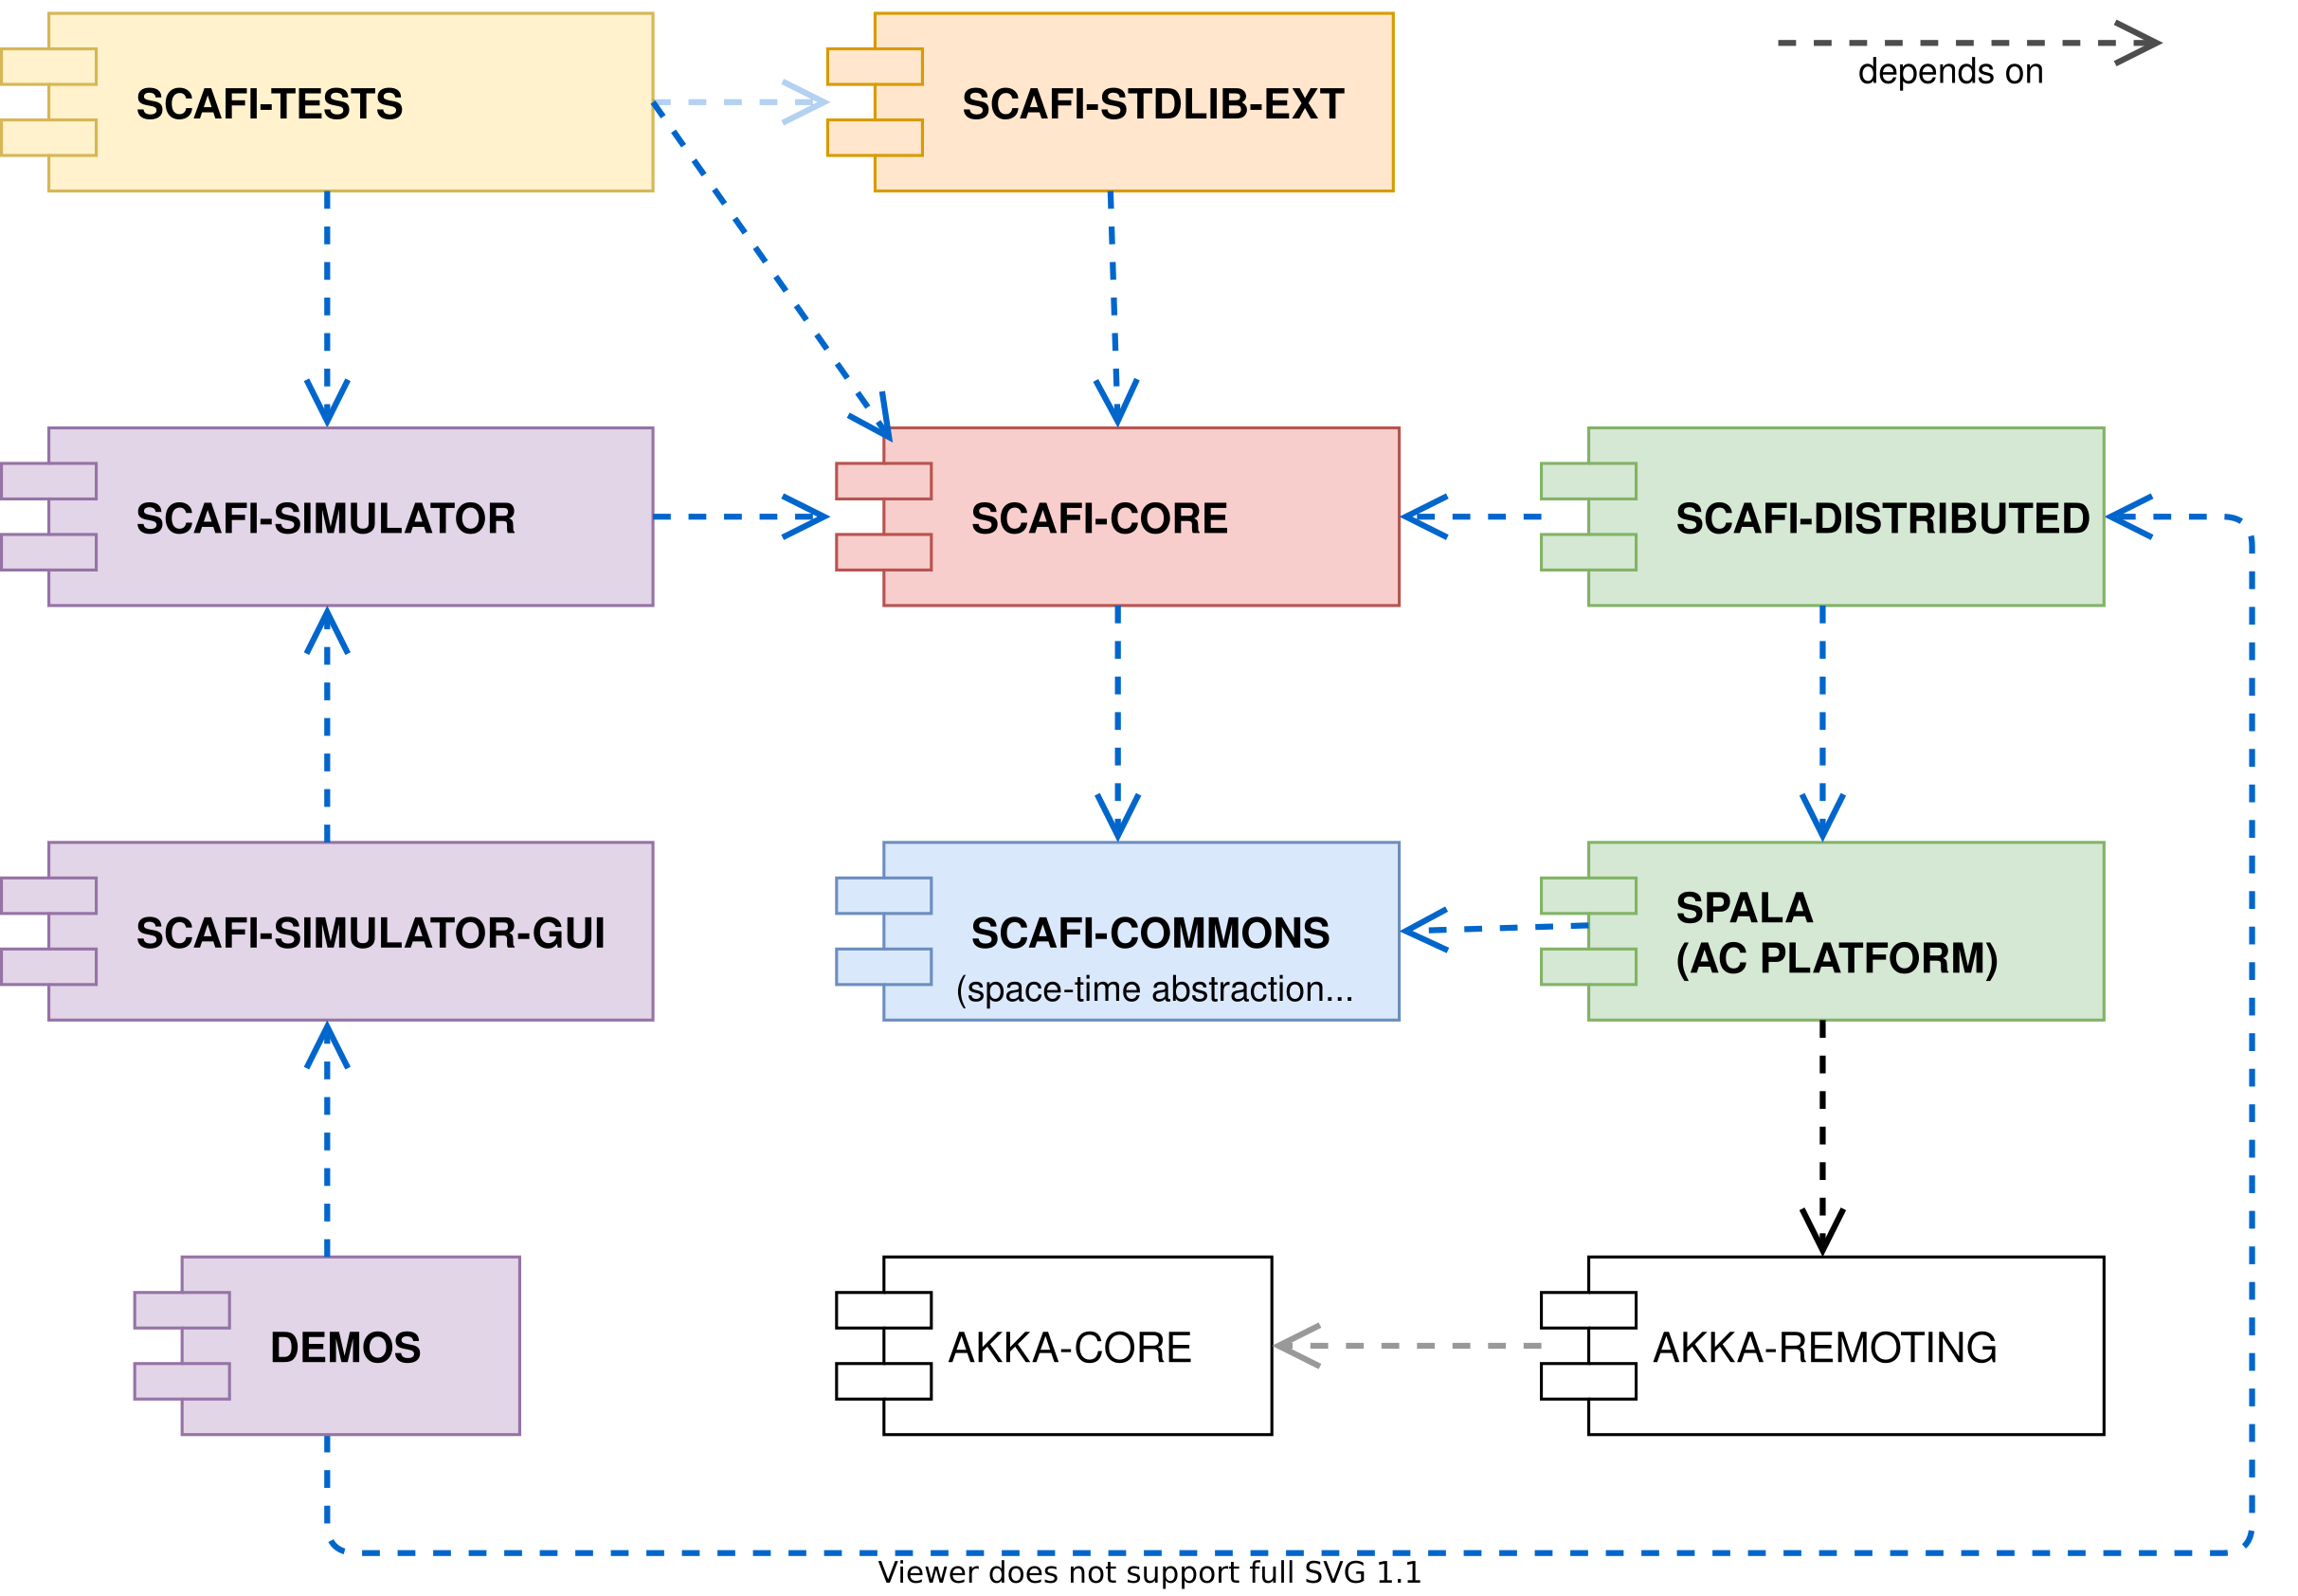
\includegraphics[width=.8\linewidth]{figures/scafi-project-org.drawio.png}
    \caption{ScaFi project organization.}
    \label{fig:scafi-project-org}
\end{figure}

Within the \texttt{core} package of the \texttt{core} module, the \texttt{Core} trait serves as the root of the family of traits.
%
It defines the set of abstract type members and traits, such as \texttt{Context}, that represents the context of the aggregate program execution.
%
A trait \texttt{Language} defines a \texttt{Constructs} trait with the core syntax of \ac{FC}, such as \texttt{rep}, \texttt{nbr}, and \texttt{foldhood}, plus additional utilities such as \texttt{mid(): ID} for retrieving the device own identifier and \texttt{sense[A](name: CNAME): A} for sensing a value from the environment.
%
Furthermore, the \texttt{RichLanguage} trait extends \texttt{Language} with additional constructs, such as \texttt{branch}, \texttt{foldhoodPlus}, and \texttt{maxHood}.
%
The \texttt{Semantics} trait implements the \ac{FC} constructs, the value tree building, and the \textit{foldhood context semantics}.
%
More insights on the foldhood semantics are provided in \cref{chap:analysis->sec:scafi-analysis->subsec:foldhood-semantics}.
%
In addition to that, the \texttt{core} module contains other packages, such as \texttt{lib} offering standard libraries, and the utilities to provide a fully-fledged aggregate program execution environment called \textit{incarnation}.
%
The \texttt{distributed} and \texttt{spala} modules enable ScaFi to run on real-world distributed applications by leveraging integration with the \textit{Akka framework}\footnote{\url{https://akka.io}} and with other supportive libraries such as \textit{Java Swing} and the \textit{Play Framework}\footnote{\url{https://www.playframework.com}}.
%
Lastly, the \texttt{simulator} and affiliated modules provide an advanced simulation suite featuring spacial and temporal simulation alongside multiple \ac{GUI} options, including a tridimensional renderer.

To use a library component in ScaFi, the user must mix in the library trait with the \texttt{AggregateProgram} base class, as shown in \cref{lst:using-libraries-in-scafi}.
%
As a consequence, all the transitive dependencies of the mixed-in libraries become visible within the scope of the program, necessitating careful construction of libraries to avoid conflicts.

\lstinputlisting[float, language=Scala, caption={Using a library component in ScaFi.}, label={lst:using-libraries-in-scafi}]{listings/scafi-using-libraries.scala}

Once the program is defined within the \texttt{main} method of the \texttt{AggregateProgram} extension, the user can execute the program on the simulator through the \texttt{Launcher}.
%
This specialized extension of Scala's \texttt{App} trait provides a \texttt{launch} method to start the simulation with one of the available \acp{GUI}.

\this aims to redesign and implement the \texttt{core} package to maintain the feasibility of integrating an equally sophisticated simulation suite while improving the overall quality of the code and the user experience.

\subsection{Foldhood semantics in ScaFi} \label{chap:analysis->sec:scafi-analysis->subsec:foldhood-semantics}

ScaFi employs the concept of a stateful \quotes{virtual machine} as its core to monitor the context of expression evaluation within the aggregate program.
%
The virtual machine not only tracks nested invocations of core constructs, but also the scope of foldhood expressions.
%
These are evaluated for each neighbor of the device, and the results of the evaluations are combined into a single value.
%
By adopting this approach, ScaFi avoids the definition of an explicit type for fields, resulting in a clean syntax but leaving the awareness of the underlying field-like nature of the foldhood semantics to the user.
%
For instance, the invalidity of expressions like \texttt{nbr{nbr{x}}} within a foldhood is something that the user must be aware of, as it is not enforced by the compiler or the virtual machine.


% ! TeX root = ../thesis-main.tex
%----------------------------------------------------------------------------------------
\chapter{Design}
\label{chap:design}
%----------------------------------------------------------------------------------------
The design of \this has been divided into three main phases.
%
In the first part, four design prototypes have been developed in order to determine the optimal user experience for three key users: the \textit{program developer}, the \textit{library developer}, and finally \textit{a new foundation researcher}, representing a novel addition to the use cases of an aggregate programming library.

In the second part, the final version of the \ac{DSL} has been designed, taking the best features from the prototypes and integrating them into a new core \ac{DSL} for \this.
%
Additionally, an execution context for aggregate programs made with \this, called \quotes{engine}, has been designed.

In the third and final part, the design process concerned the execution engine and the simulator.

The first and second part cover requirements \textit{F.1}, \textit{F.3}, \textit{F.6}, \textit{F.7}, and \textit{T.1}, while the third covers requirement \textit{F.5} from \Cref{chap:analysis->sec:requirement-analysis}.

\section{Designing a scalable internal Domain Specific Language} \label{chap:design->sec:dsl}

The process of designing a new core \ac{DSL} for \this has been carried out through rapid prototyping of four competing designs of different \acp{DSL}, each coming with a set of advantages and disadvantages, highlighted using code snippets for every key user.
%
Prototipation has been necessary to explore the design space and to understand the trade-offs between different design options, as well as to test in practice the interactions of different combinations of language features.
%
For each of the four prototypes, a brief description of the design choices and the programming experience is provided, followed by the final design described in \Cref{chap:design->sec:final-dsl}.
%
Each prototype is named after the Scala 3 feature it is mainly based on, and each aims to separate the definition of the syntax from the definition of the semantics, and separate the definition of the semantics from the actual implementation.
%
This way, more than one semantics can be defined for the same syntax, and more than one implementation can be defined for the same semantics, allowing for more flexible customization and composition.
%
While the \ac{XC}~\cite{xc} is the only semantics considered for implementation within the scope of \this, the design should be flexible enough for potential future \quotes{calculi} to be implemented as alternative foundations.
%
It is worth noting that there exists a subtle distinction between the semantics and syntax of the same formal calculus in practice.
%
In the case of \ac{XC}, both the syntax and the semantics consist of two methods, \texttt{branch} and \texttt{exchange}.
%
The difference lies in the role of the two methods in the two contexts: in the syntax, they are constructs that the programmer uses to write programs, and should be treated as an \ac{API} at all effects, while in the semantics, they are constructs that the programmer uses to implement all the supported syntaxes \ac{API}, meaning they are not part of an \ac{API} used by aggregate programs and are focused on being as complete and simple to implement as possible.
%
For instance, the \texttt{exchange} method of the \texttt{ExchangeCalculusSyntax} trait is focused on its usage experience, attempting to imitate the syntax provided in the paper, meanwhile the \texttt{xcexchange} method of the \texttt{ExchangeCalculusSemantics} has \texttt{protected} visibility and its signature provides only the most complete and expressive version of the \texttt{exchange} primitive presented in the paper~\cite{xc}.

Each of the four prototypes retains the separation between syntax definitions, semantic definitions, syntax support declaration, and semantics implementations, and considers the programmer experience of all the three key users.
%
For brevity, only the most relevant advantages and disadvantages are highlighted, and the full code of the prototypes is available in the project repository git history, under the git tag \texttt{experiments}\footnote{\url{https://github.com/ldeluigi/scafi-xc/tree/experiments}}, after which the code got removed to avoid confusion with the final design.


\subsection{Prototype 1: Extension Methods} \label{chap:design->sec:dsl->subsec:prototype-1-extension-methods}

In this design, an \texttt{AggregateFoundation} base trait defines a common syntax for all the aggregate programming foundations, such as the existence of a type called \texttt{AggregateValue[T]} that represents a collection of values coming from neighboring devices, including self.
%
The \texttt{AggregateFoundation} trait also defines a set of \textit{abstract extension methods} that provide basic functionalities for aggregate values, such as \textit{lifting} for composition and mapping, \textit{folding} for reduction, methods for retrieving the value for the current device or exclude the current device, mimicking the functionalities of the \texttt{foldhood} and \texttt{foldhoodPlus} of ScaFi, as shown in \Cref{lst:prototype-1-aggregate-foundation}.
%
In the example, the source of the \texttt{Liftable} and \texttt{Foldable} type classes is included for completeness, but they are not part of the \texttt{AggregateFoundation} source file as they are located in the \texttt{commons} module.

\lstinputlisting[float, language=Scala, caption={Prototype 1 - Aggregate Foundation and helper type classes.}, label={lst:prototype-1-aggregate-foundation}]{listings/prototype-1-aggregate-foundation.scala}

By defining an abstract type member \texttt{AggregateValue[T]}, semantics like \ac{XC} can override it to model any kind of specific interface, such as \textit{NValues}, on top of which they can provide any additional behavior and syntax, following the pattern of \textit{family polimorphism}.
%
Implicitly, this design abandons the \quotes{field-transparent} semantics of the \texttt{foooldhood*} methods of ScaFi in favor of having explicit \textit{field} types, similarly to FCPP (\Cref{chap:state-of-the-art->sec:fcpp}) and the \ac{XC} \ac{DSL} experiment (\Cref{chap:state-of-the-art->sec:xc-experiment}).
%
Nevertheless, a semantics design that replicates that lost feature can still be implemented with an extension of \texttt{AggregateFoundation} that provides a \texttt{foldhood} construct that works the same as the \texttt{foldhood*} methods of ScaFi.

\textit{Aggregate Semantics} such as \texttt{ExchangeCalculusSemantics} are defined as a trait that extends \texttt{AggregateFoundation}.
%
A semantics trait can provide a concrete type for the abstract type member \texttt{AggregateValue[T]}, even if the type refers to a trait and not a concrete implementation.

For instance, the \texttt{ExchangeCalculusSemantics} provides a concrete implementation for \texttt{AggregateValue[T]} corresponding to \texttt{NValues[ID, T]}, where \texttt{ID} is an abstract type member for device identifiers.
%
Additionally, the semantics provides an abstract given instance of \texttt{CanEqual[ID, ID]} to provide equality comparisons between device identifiers, as well as the core \ac{XC} constructs: \texttt{xcexchange} and \texttt{xcbranch}, corresponding to the \texttt{exchange} primitive and the domain branching behavior of \ac{XC}.
%
These core constructs of the semantics are protected in visibility because they are meant to be invoked only through a facade that corresponds to one or more syntax of a \textit{calculus}, whereas abstract given instances are public as they are meant to be available to libraries that depend on a specific semantics.
%
The syntaxes for both \ac{FC} and \ac{XC} are shown in \Cref{lst:prototype-1-syntaxes}, and the \ac{XC} semantics is shown in \Cref{lst:prototype-1-exchange-calculus-semantics}.
%
Finally, \Cref{lst:prototype-1-syntaxes-impl} shows the implementation of the syntaxes in terms of the \ac{XC} semantics.

One notable feature of having a facade defined using extension methods is that the compatibility layer between a semantic and a syntax is provided through the implementation of a given instance, much like a written proof that a syntax can be obtained extending a given semantics.
%
The proof can \texttt{summon} other given instances of supported syntax in order to define a proof dependent on another proof, as shown in \Cref{lst:prototype-1-syntaxes-impl}.
%
Another significant feature is the possibility to import dependencies and preferred syntax/facade with an \texttt{import} statement at the beginning of the file, instead of having to mix in traits like in ScaFi.
%
Additionally, this design allows implementing a new library by simply writing new extension methods of a generic language \texttt{L} that extends \texttt{AggregateFoundation} and the required other syntaxes, as shown in \Cref{lst:prototype-1-usage-lib}.
%
This allows libraries to be singleton objects, imported where needed with a top-level \texttt{import} statement.
%
One hidden feature of this design is the possibility to hide, by default, transitive library dependencies, something that ScaFi could not allow because it used a mixin composition where every library was a trait that mixed in other traits, thus exposing all the dependencies of the mixed-in traits.

\lstinputlisting[float, language=Scala, caption={Prototype 1 - Syntax definitions.}, label={lst:prototype-1-syntaxes}]{listings/prototype-1-syntaxes.scala}
\lstinputlisting[float, language=Scala, caption={Prototype 1 - Exchange Calculus Semantics.}, label={lst:prototype-1-exchange-calculus-semantics}]{listings/prototype-1-exchange-calculus-semantics.scala}
\lstinputlisting[float, language=Scala, caption={Prototype 1 - Syntax implementations in terms of the exchange semantics.}, label={lst:prototype-1-syntaxes-impl}]{listings/prototype-1-syntaxes-impl.scala}

Even though this design proves to be very flexible and extensible, it has a few drawbacks.
%
The most important one is the impossibility of invoking an extension method without the \quotes{\texttt{.}}, having at best to invoke constructs on \texttt{this}, as in \Cref{lst:prototype-1-usage}.
%
The next prototypes focus on overcoming this limitation at any cost, even if it means losing some of the flexibility and clarity of the design, in order to provide empirical evidence of the trade-offs between the different design choices.

\lstinputlisting[float, language=Scala, caption={Prototype 1 - Example usage by an aggregate program developer.}, label={lst:prototype-1-usage}]{listings/prototype-1-usage.scala}
\lstinputlisting[float, language=Scala, caption={Prototype 1 - Example usage by a library developer.}, label={lst:prototype-1-usage-lib}]{listings/prototype-1-usage-lib.scala}


\subsection{Prototype 2: Context parameter in constructors} \label{chap:design->sec:dsl->subsec:prototype-2-implicit-parameter-in-constructors}

Even though the second prototype is based on the use of a context parameter that passes a semantics instance down to every construct invocation, the folding and lifting functionalities are provided through abstract given instances of type classes declaring extension methods, as per prototype 1.
%
Libraries, as well as core syntaxes, are defined as classes and traits, respectively, that take a context parameter of type \texttt{L}, short for \texttt{Language}, that must be a subtype of \texttt{AggregateFoundation}, as shown in \Cref{lst:prototype-2-syntax}.
%
Libraries dependent on other libraries must either instantiate their dependencies or require a context parameter that provides them, as shown in \Cref{lst:prototype-2-usage-lib}.
%
This approach has the side effect that the type member \texttt{AggregateValue} present in the \texttt{AggregateFoundation} is seen as a different type for every dependent method of every library, thus making passing an aggregate value from a library method to another impossible.
%
This forced each semantics, library, and syntax to have a generic type constructor parameter \texttt{AV[\_]} that generalizes and uniformizes the type of the aggregate value for all the dependencies, making them compatible again.
%
\Cref{lst:prototype-2-usage-lib} also shows how this design, with the additional cost of a static \texttt{import} for dependencies methods and given instance, allows to invoke constructs such as \texttt{branch} or \texttt{distanceTo} with having to use the \texttt{.} operator and the same applies to user programs.

\lstinputlisting[float, language=Scala, caption={Prototype 2 - Field Calculus syntax definition.}, label={lst:prototype-2-syntax}]{listings/prototype-2-syntax.scala}
\lstinputlisting[float, language=Scala, caption={Prototype 2 - Example usage by a library developer.}, label={lst:prototype-2-usage-lib}]{listings/prototype-2-usage-lib.scala}

Having to explicitly import the methods from dependencies inside every library of programs, added to the necessity of instantiating libraries, makes this design very cumbersome to use.
%
The next prototype attempts to improve the usability by returning to libraries defined as singleton objects, having each construct take the context parameter that were in the library class constructor in this prototype.


\subsection{Prototype 3: Implicit parameter in methods} \label{chap:design->sec:dsl->subsec:prototype-3-implicit-parameter-in-methods}

This prototype design shares some similarities with the previous one, but it has a different approach to the problem of passing the semantics instance to the constructs, and to dealing with library dependencies.
%
In this design, libraries are singleton objects, where each method takes a context parameter for the semantics and a context parameter for every syntax needed as a dependency, as shown in \Cref{lst:prototype-3-usage-lib}.
%
Alternatively, a library method can instantiate its syntax dependencies and only take a context parameter for the semantics, in a similar way to the previous prototype.
%
Even though the issue of library dependencies is solved, syntax dependencies are still cumbersome to use and still require static imports inside the body of the methods to invoke the constructs without the \texttt{.} operator.
%
In addition to that, \texttt{AggregateFoundation} still needs the generic aggregate value type constructor parameter to make syntax dependencies compatible with each other.

\lstinputlisting[float, language=Scala, caption={Prototype 3 - Example usage by a library developer.}, label={lst:prototype-3-usage-lib}]{listings/prototype-3-usage-lib.scala}

The last prototype represents a return to the original mixin-oriented design used in ScaFi and its purpose is closer to a comparison baseline rather than a design alternative, but it is still useful for the last design phase where the best features of all the prototypes will be cherry-picked and combined.

\subsection{Prototype 4: Mixin composition} \label{chap:design->sec:dsl->subsec:prototype-4-mixin-composition}

In this design, the \texttt{AggregateFoundation} trait is the same as in prototype 1 (see \Cref{lst:prototype-1-aggregate-foundation}), without the need for the generic type constructor for aggregate values, because syntaxes, semantics, and the foundation are meant to become part of the same type hierarchy, and a type member for aggregate values will be the same for all the mixed-in traits.
%
For instance, given a semantics such as \texttt{ExchangeCalculusSemantics}, giving proof for the support for a syntax means to define a trait to be mixed in with the semantics, that implements the syntax in terms of the semantics.
%
Libraries are defined, like in ScaFi, with mixin traits that declare their dependencies using self-type annotations, as shown in \Cref{lst:prototype-4-usage-lib}.

The main advantage of this design is the possibility to invoke constructs without the \texttt{.} operator, as shown in \Cref{lst:prototype-4-usage-lib}, while the main disadvantage is the need to inherit from all the transitive dependencies together in the program class, and having to honor a global construct naming consistency both in all the libraries and in the semantics implementation.

\lstinputlisting[float, language=Scala, caption={Prototype 4 - Example usage by a library developer.}, label={lst:prototype-4-usage-lib}]{listings/prototype-4-usage-lib.scala}

\section{Final design of the core DSL} \label{chap:design->sec:final-dsl}

Taking inspiration from the best features of all the prototypes, the final design was developed and showcased with a presentation in front of the research group, which provided positive feedback on the resulting user experience.
%
The final design consists of an \texttt{AggregateFoundation} similar to prototypes 1 and 4, with core syntaxes and libraries defined as traits for a mixin composition.
%
The twist is that libraries are instead defined as singleton objects, able to be imported with a top-level \texttt{import} statement, without having visibility on transitive dependencies and without having to mix them in together with the semantics in the program class.
%
The disadvantage of this design would have been the different invocation syntax for library constructs versus core syntax constructs such as \texttt{nbr} and \texttt{rep}.
%
This disadvantage has been overcome by defining a facade library for every core syntax, hiding the \quotes{\texttt{language.}} prefix necessary for invoking core syntax constructs, with the small cost of having to write a facade library for every future syntax developed by researchers.
%
An \ac{UML} diagram of the final model for the foundation is shown in \Cref{fig:final-design-foundation-diagram}.

\begin{figure}
    \centering
    \caption{Final design: \ac{UML} diagram of the \texttt{AggregateFoundation}.}
    \label{fig:final-design-foundation-diagram}
    \bigskip
    \resizebox{\linewidth}{!}{
        \input{diagrams/final-design-foundation/Final Design Foundation.latex}
    }
\end{figure}

\Cref{fig:final-design-exchange-calculus-semantics-diagram} shows the \ac{UML} diagram of the \texttt{ExchangeCalculusSemantics} mixin composition, which is the only semantics implemented for the scope of this project.

\begin{figure}
    \centering
    \caption{Final design: \ac{UML} diagram of the \texttt{ExchangeCalculusSemantics} mixin composition.}
    \label{fig:final-design-exchange-calculus-semantics-diagram}
    \bigskip
    \resizebox{\linewidth}{!}{
        \input{diagrams/final-design-semantics/Final Design Semantics.latex}
    }
\end{figure}

Thanks to this design, the gradient construct, also known as \texttt{distanceTo}, can be defined to work with any aggregate semantics that supports the field calculus syntax, and thanks to Scala context bounds it can also be defined to work with any numeric type that supports an upper bound, such as \texttt{Double}.
%
The resulting code for the \texttt{distanceTo} construct is shown in \Cref{lst:distance-to}, which resembles the syntax of the prototype \ac{DSL} of \Cref{lst:gradient-distance-xc-scala2-dsl}.
%
The provided snippet demonstrates how this design effectively achieves the goals pursued by the other design prototypes:
\begin{itemize}
    \item invocation of library and core constructs without the \texttt{.} operator;
    \item declaration of library dependencies with top-level imports, that hide transitive dependencies;
    \item generic definition of the constructs for high reusability;
    \item clean declaration of the core syntax dependencies, using a \quotes{\texttt{language}} context parameter and intersection types;
    \item possibility to resolve naming conflicts with import aliases;
    \item reuse of all the libraries and programs dependent on a set of syntaxes by re-implementing them through the next generation of aggregate programming calculi;
\end{itemize}

\lstinputlisting[float, language=Scala, caption={Final design - \texttt{distanceTo} implementation in the \texttt{GradientLibrary}.}, label={lst:distance-to}]{listings/distance-to.scala}

\subsection{Design of the XC operational semantics} \label{chap:design->sec:final-dsl->subsec:exchange-calculus-semantics-design}

By abstracting common features of aggregate programming languages such as \ac{FC} and \ac{XC} into the \texttt{AggregateFoundation} trait, the \texttt{ExchangeCalculusSemantics} can focus on the peculiarities of the \ac{XC} semantics, such as NValues and the \texttt{exchange} primitive.
%
\texttt{AggregateFoundation} provides an abstract definition of an \texttt{AggregateValue} type, with the only feature to be iterable.
%
The reason is that whatever the next aggregate calculus semantics will be, it is expected to provide some kind of notion of field, which should allow iterating over values from neighbors, including self.
%
Additionally, \texttt{AggregateFoundation} provides the \ac{API} to exclude the value for self from an \texttt{AggregateValue}, as well as to retrieve the value for self only, using extensions method inspired by the \ac{XC} \ac{DSL} experiment of \Cref{chap:state-of-the-art->sec:xc-experiment}.
%
Referencing self has an important role in aggregate programs, and it was put here to provide all libraries and programs with that feature.
%
Finally, \texttt{AggregateFoundation} provides the means to combine and map aggregate values with the \texttt{lift} operator and the \texttt{map} extension method.
%
This is a necessary difference from the formal calculi, where aggregate values such as NValues or fields allow to be treated as their underlying generic type, and are transparent when combined or mapped as if they were local values.
%
For example, in \ac{XC}, an expression $e$ written to work with local values of type \texttt{T} can be used with an aggregate value of type \texttt{NValues[T]} without any modification.
%
In Scala, instead, this is not possible, and operations on local values need to be \textit{lifted} to work on aggregate values too.
%
Unary operations have to be lifted too and work as the mapping function \texttt{f: A => B} for the \texttt{map} extension method available on an \texttt{AggregateValue[A]}.
%
As mentioned in the previous section, abstracting common features into a common foundation for all the semantics allows the reuse of all the libraries and programs depending on those features, while also retaining the possibility to re-implement differently in a new aggregate calculus semantics.

To allow the definition, in the future, of an aggregate calculus without explicit device identifiers exposed in the \ac{API}, all the features related to explicit device identifiers in the calculus have been grouped and modeled as an optional mixin called \texttt{DeviceAwareAggregateFoundation}.
%
The mixin defines an abstract type member \texttt{DeviceId} and the means to compare them with \texttt{==}, that is a given instance of \texttt{CanEqual[DeviceId, DeviceId]}.
%
In addition to that, it provides two abstract methods, one called \texttt{self} that returns the device identifier of the current device, and another called \texttt{device} that returns an aggregate value of device identifiers, including self, which is always known thanks to the network and it doesn't need to be computed with, for example, a \texttt{nbr(self)} invocation.

Therefore, the \texttt{ExchangeCalculusSemantics} is left only with the definitions of its specific features, which are NValues additional operation on aggregate values, automatic conversion from local values and NValues, the core constructs \texttt{exchange}, here called \texttt{xc}, and \texttt{branch}, called \texttt{br}, to avoid conflicts with their counterparts defined in the implemented syntaxes.
%
The signature of the \texttt{xc} method has been simplified to simplify its implementation, written only in its complete form with both the \texttt{return} and \texttt{send} values explicitly passed as a couple, whereas the \texttt{exchange} method of the syntax allows different call signatures to imitate the syntax of the paper~\cite{xc}, as shown in \Cref{lst:exchange-syntax}.

\lstinputlisting[float, language=Scala, caption={Supported syntaxes for invoking the \texttt{exchange} primitive.}, label={lst:exchange-syntax}]{listings/exchange-syntax.scala}

The concrete implementation of the \ac{XC} operational semantics is discussed partly in the next section, and partly in \Cref{chap:implementation->sec:xc-ops}.

\subsection{The Engine} \label{chap:design->sec:final-dsl->subsec:engine}

An \texttt{Engine} has been designed to be able to execute aggregate programs that use an instance of the \ac{XC} semantics trait as a context parameter.
%
The \texttt{Engine} offers a method called \texttt{cycle} which implements all the steps to be executed in a single round of an aggregate program.
%
The steps can be summarized into the following:
\begin{enumerate}
    \item instantiation of the semantics, whose implementation is called \texttt{Context}, using information coming from the \texttt{Network}, such as inbound messages and the device identifier;
    \item execution of the aggregate program, which is a function that takes the \texttt{Context} as a context parameter and returns a \texttt{Result}, which is the result of the evaluation of the aggregate program;
    \item collection of the \texttt{Export}, which is a bundle containing all the outbound messages;
    \item sending of the \texttt{Export} to the \texttt{Network}, which will deliver the messages to the intended recipients.
\end{enumerate}
%
A \texttt{Context} is defined as an interface that takes inbound messages as input, called \texttt{Import}, gets altered by the aggregate program round of execution, and produces outbound messages as output, called \texttt{Export}.
%
More information about the implementation of a \texttt{Context} for the \ac{XC} semantics can be found in \Cref{chap:implementation->sec:xc-ops}.
%
An \texttt{Import} is defined as an alias for a map from device identifiers to generic values, which for the only implemented context correspond to \textit{value trees}.
%
A \texttt{ValueTree} is an \ac{ADT} containing the values exchanged between devices coupled with their path in the \ac{AST} of the aggregate program, as described in the \ac{XC} paper~\cite{xc}.
%
Here a \texttt{Path} is defined as an alias for a \texttt{List} of generic tokens so that every implementation of a semantic can control which type of token defines a location inside the \ac{AST} of the aggregate program.
%
An \texttt{Export} instead is defined as an alias for a \texttt{MapWithDefault}, because it can send a dedicated message to a known neighbor and a default message to every other new neighbor of the device.
%
The \texttt{Network} is responsible for properly dispatching the messages to the intended recipients and is pictured with \ac{UML} in \Cref{fig:engine-network-diagram}.

\begin{figure}
    \centering
    \caption{The engine: \ac{UML} diagram of the \texttt{Network} interface.}
    \label{fig:engine-network-diagram}
    \bigskip
    \resizebox{\linewidth}{!}{
        \input{diagrams/network/Network.latex}
    }
\end{figure}

In summary, the \texttt{Engine}, uses a \texttt{ContextFactory} to repeatedly instantiate a new \texttt{Context} for every cycle of the aggregate program execution, executes the program against the context, and finally sends the result to the network.
%
An \ac{UML} diagram of the \texttt{Context} and the \texttt{Engine} can be found in \Cref{fig:engine-diagram}.

\begin{figure}
    \centering
    \caption{The engine: \ac{UML} diagram of the \texttt{Context} interface and the \texttt{Engine} class.}
    \label{fig:engine-diagram}
    \bigskip
    \resizebox{\linewidth}{!}{
        \input{diagrams/engine/Engine.latex}
    }
\end{figure}


\section{Network-based sensors} \label{chap:design->sec:network-based-sensors}

In general, sensors and actuators are not part of the \ac{DSL} of \this.
%
In ScaFi, sensors are modeled as a key-value dictionary, from \texttt{String} to \texttt{Any}, that casts the value to the expected type.
%
To improve the type safety and to have less error-prone sensor access, in this design sensor and actuator design and implementation are left to the user, that can provide them in three main ways:
\begin{enumerate}
    \item by implementing an external library that interacts with the sensor and actuator hardware, which gets invoked by the aggregate program;
    \item by extending the \texttt{Context} implementation with additional, type-safe sensor and actuator methods, invoked in the aggregate program in the form \texttt{ctx.sensorName()} or \texttt{summon[ContextImpl].sensorName()};
    \item by both extending the \texttt{Context} and implementing an external library as its facade, to provide an \ac{API} with static method signatures that can be invoked in the aggregate program, in line with the style of the \ac{DSL}.
\end{enumerate}
%
This design choice has been made to keep the \ac{DSL} as simple as possible and to allow the user to choose the best way to interact with the sensor and actuator hardware, as well as to allow the user to choose the best way to model the sensor and actuator data, which can be very different from one application to another.
%
Nevertheless, network-based sensors, which are sensors whose measured values differ for every visible neighbor, represent a special case.
%
These sensors must either be implemented following the second or the third way of the list above, because a measurement must return an \texttt{AggregateValue[T]} where \texttt{T} is the type of the measurement and the aggregate value contains a measurement for every visible neighbor, including self.

The standard library included in the \texttt{core} module provides a network-based sensor called \texttt{DistanceSensor}, due to its importance in common aggregate programs.
%
In ScaFi, the corresponding construct is called \texttt{nbrRange}.
%
If an aggregate context implements the \texttt{DistanceSensor[N: Numeric]} trait, \texttt{senseDistance: N} is available to be invoked in the aggregate program, and it returns a value of type \texttt{AggregateValue[N]} containing the distance to every visible neighbor, including self.
%
The availability of the distance sensor in the context enables the invocation of library constructs based on that, such as the \texttt{sensorDistanceTo} of the \texttt{GradientLibrary} which uses the sensors as metric for the distance to the neighbors.
%
The distance sensor is generic on the type of the measurement, as long as it is a numeric type, to allow for different configurations, such as measuring with floats, integers, or custom types that provide a \texttt{Numeric} given instance.


\section{The simulator}

The simulator module serves both as a tool for developers to test their programs in a controlled environment and as a fundamental component for the acceptance tests.
%
For the scope of this project, the simulator has been designed to be as simple as possible, providing a minimal set of functionalities that are enough to test the \ac{DSL} and the libraries developed for it.
%
As a result, the simulator is deterministic, with discrete time, and models neighborhoods as a map from device identifiers to a set of device identifiers.
%
Nevertheless, the simulator implements basic real-world network phenomena such as message loss and delay, as well as customizable message retention time and device reboot/failures.
%
Inside tests, a \textit{deterministic} simulator allows control of every aspect of the aforementioned features through the use of policies, implementing the strategy pattern.
%
In addition to that, in manual tests, a \textit{random} simulator could be used.
%
The random simulator allows the generation of randomized device networks and randomized policies to simulate an environment closer to the internet, following a set of given parameters for the probability distributions used in the implementation.
%
This is particularly useful to test the self-healing, self-organizing properties of aggregate programs.
%
Tests can be reproduced deterministically even in the random simulator thanks to the \texttt{seed} parameter that controls the generation of pseudo-random numbers.
%
The resulting \ac{UML} diagram of the simulator module design is shown in \Cref{fig:simulator-uml}.

\begin{figure}
    \centering
    \caption{\ac{UML} diagram of the \texttt{simulator} module.}
    \label{fig:simulator-uml}
    \bigskip
    \resizebox{\linewidth}{!}{
        \input{diagrams/simulator/Simulator.latex}
    }
\end{figure}


% ! TeX root = ../thesis-main.tex
%----------------------------------------------------------------------------------------
\chapter{Implementation}
\label{chap:implementation}
%----------------------------------------------------------------------------------------

This chapter documents the implementation details of the models and libraries designed, as well as additional tools and extensions developed as research experiments and proof of concepts.
%
The implementation of the \texttt{core} and \texttt{simulator} modules has no external, third-party dependencies apart from the Scala standard library, thus satisfying the requirement \textit{T.7} from \cref{chap:analysis->sec:requirement-analysis}.
%
In particular, the chapter covers the implementation of an experimental \texttt{FoldhoodLibrary}, that demonstrates the expressiveness of the \this design by implementing an \ac{API} for \texttt{foldhood} and \texttt{foldhoodPlus} similar to the original ScaFi, and the prototype of a different implementation of the \texttt{AggregateFoundation} trait, which adds compile time assertions on the user code to prevent common mistakes and improve the quality of aggregate programs, at the expense of more complicated signatures of library methods, following requirement \textit{F.8} from \cref{chap:analysis->sec:requirement-analysis}.
%
The chapter also covers the integration of \this with the Alchemist simulator (requirement \textit{F.4} from \cref{chap:analysis->sec:requirement-analysis}), which enables graphical and more realistic simulations, as well as additional proof of the functionality of \this.

\section{Implementation of the XC operational semantics} \label{chap:implementation->sec:xc-ops}

The implementation of the operational semantics as described in paper\cite{xc} follows the design of \cref{chap:design->sec:final-dsl->subsec:exchange-calculus-semantics-design} by defining a concrete class that inherits from \texttt{ExchangeCalculusSemantics}.
%
Given that the same class serves as context for the execution of aggregate programs' rounds, following the engine design of \cref{chap:design->sec:final-dsl->subsec:engine}, it implements the \texttt{Context} interface too.

The implementation is named \texttt{BasicExchangeCalculusContext}, because it is meant to provide a simple yet readable and reliable implementation, without pursuing premature optimizations or additional features.
%
A more advanced implementation could be developed in the future, maybe specifically tailored to some destination platform or network implementation.
%
In order to maximize the reusability of its code, the logic and behavior that compose the operational semantics has been broken down into several mixin layers, with their dependencies declared through self-type annotations and abstract members.
%
These mixin layers have been organized into two packages based on their reusability: \texttt{context.common} with the most general and reusable mixins, and \texttt{context.exchange} with the mixins that are specific to the exchange calculus, as shown in \cref{fig:context-mixins-common,fig:context-mixins-exchange}.

\begin{figure}
    \centering
    \caption{Exchange Calculus context mixins: \ac{UML} diagram of the mixin layers in package \texttt{common}, stripped of transitive dependencies.}
    \label{fig:context-mixins-common}
    \bigskip
    \resizebox{\linewidth}{!}{
        \input{diagrams/context-mixins/Context Mixins - Common.latex}
    }
\end{figure}

\begin{figure}
    \centering
    \caption{Exchange Calculus context mixins: \ac{UML} diagram of the mixin layers in package \texttt{exchange}, stripped of transitive dependencies.}
    \label{fig:context-mixins-exchange}
    \bigskip
    \resizebox{\linewidth}{!}{
        \input{diagrams/context-mixins/Context Mixins - Exchange.latex}
    }
\end{figure}


\subsection{The stack-based semantics implementation}

Without using Scala 3 macros everywhere an aggregate expression is written, the \ac{AST} of an aggregate program is not directly available to the semantics implementation.
%
Consequently, the semantics implementation has to track the invocation of its primitives into an explicit stack-like \ac{ADT}, while building the \texttt{Export} value tree using the paths traced by the stack.
%
If a primitive invocation is nested inside another, the invocation trace is pushed into the stack, and the nested expression is evaluated, potentially growing the stack but leaving it unchanged at the end of the evaluation, and then the trace is popped from the stack.
%
This logic is implemented in the \texttt{scope} method of \texttt{StackSemantics} and is employed by the \texttt{xc} implementation of \texttt{exchange.ConstructsSemantics}.
%
For instance, the program in \cref{lst:value-tree-example}, at the first execution round with the \texttt{BasicExchangeCalculusContext}, would produce the value tree in \cref{fig:value-tree-example}.

\lstinputlisting[float, language=Scala, caption={Example of aggregate program that produces the value tree in \cref{fig:value-tree-example}.}, label={lst:value-tree-example}]{listings/value-tree-program.scala}

\begin{figure}
    \centering
    \caption{Example of value tree produced by the program in \cref{lst:value-tree-example}.}
    \label{fig:value-tree-example}
    \bigskip
    \resizebox{0.5\linewidth}{!}{
        \input{diagrams/value-tree/Value Tree Example.latex}
    }
\end{figure}

Alignment is implemented by comparing the current stack with the neighbor's value trees: if a path prefix is in common, the device is aligned with the given neighbor.
%
In order to distinguish \texttt{exchange} invocations that are not part of the same conditional branch, it is necessary that the \texttt{branch} construct is invoked in place of Scala's \texttt{if}, and that the \texttt{branch} construct is implemented to push a branch identifier into the stack using the scope method, thus misaligning devices who took different branches.
%
A known limitation and pitfall of this solution, besides making programmers understand the need to use \texttt{branch} instead of \texttt{if}, is boolean short-circuiting, which behaves similarly to the \texttt{if} construct, in the sense that it can happen to skip the evaluation of some exchange calls without tracing the conditional branch in the stack.
%
When that happens, the resulting behavior is unpredictable and will probably lead to runtime errors.

\texttt{InboundMessagesSemantics} is responsible for providing the set of currently aligned devices as well as retrieving the values corresponding to the current traced path from their value trees.
%
\texttt{OutboundMessagesSemantics} is responsible for building the export value tree using the current path and the values passed to the \texttt{sendMessages} method.
%
Once the program round has completed, and the \texttt{Engine} asks for the \texttt{Export} value tree, the sent messages are reorganized into a different value tree for every known neighbor, plus the current device, because memory is modeled as a self-message, and a default value tree for every new neighbor that appears during sleep time.
%
This is the reason why the \texttt{Export} is an alias for a \texttt{MapWithDefault} while the \texttt{Import} is an alias for a \texttt{Map}, with both \ac{ADT} immutable.

Inside a value tree, values of different types are stored together under a common type, and they need to be converted back to their original types when extracted from the tree.
%
For this reason, \texttt{MessageSemantics} offers two methods, \texttt{open} and \texttt{close}, responsible for the conversion from and to the common type, defined with an abstract type member called \texttt{Envelope}.
%
In a real-world distributed system, an \texttt{Envelope} could be a sequence of bytes, containing the serialized stream from shared objects.
%
For the scope of \this, all the simulations are executed using the \texttt{MessageSemantics.Basic} implementation, which simply casts the values to and from \texttt{Any}, which works because the simulations are run in a single JVM, and the \texttt{Any} type is the root of the Scala type hierarchy.

\section{The build system}

Following the requirements listed in \cref{chap:analysis->sec:requirement-analysis}, the chosen build system for the project is \ac{SBT}, in particular version \texttt{1.9.8}, following requirement \textit{T.3} from \cref{chap:analysis->sec:requirement-analysis}.
%
The build tool has been customized with the following plugins:
\begin{itemize}
    \item \texttt{sbt-scalafix} to lint the code with \textit{scalafix}, further explained in \cref{chap:evaluation->sec:code-style}, following requirement \textit{T.6} from \cref{chap:analysis->sec:requirement-analysis};
    \item \texttt{sbt-scalafmt} to lint the code with \textit{scalafmt}, further explained in \cref{chap:evaluation->sec:code-style}, following requirement \textit{T.6} from \cref{chap:analysis->sec:requirement-analysis};
    \item \texttt{sbt-scalajs} and \texttt{bt-scalajs-crossproject} to cross-build the project for \textit{JavaScript} with \textit{scala-js}, following requirement \textit{T.4} from \cref{chap:analysis->sec:requirement-analysis};
    \item \texttt{sbt-scala-native} and \texttt{sbt-scala-native-crossproject} to cross-build the project for \textit{native} with \textit{scala-native}, following requirement \textit{T.5} from \cref{chap:analysis->sec:requirement-analysis}.
\end{itemize}
%
In addition to that, the Dotty compiler has been customized with flags that enhance the quality of the code, such as the aforementioned \textit{explicit nulls} and \textit{multiversal equality}, but also enforcement for indentation over curly braces style, warnings as errors, safe initialization checks, warnings on value discards, and more (requirement \textit{T.2} from \cref{chap:analysis->sec:requirement-analysis}).

\section{The \quotes{FoldhoodLibrary}} \label{chap:implementation->sec:foldhood-library}

As a proof of concept of the expressiveness of the \this design, an experimental library has been developed, called \texttt{FoldhoodLibrary}, which provides an \ac{API} for the \texttt{foldhood} and \texttt{foldhoodPlus} constructs as defined in the original ScaFi library, representing in a way an internal \ac{DSL} written in terms of another.
%
The library works for any aggregate context that supports the \texttt{FieldCalculusSyntax}, and implements \texttt{foldhood}, \texttt{foldhoodPlus}, \texttt{nbr}, and \texttt{nbrRange} for contexts that also support \texttt{DistanceSensor}.
%
The resulting \ac{API} can be seen used in \cref{lst:foldhood-library-usage},
where \texttt{nbr} is not the same as the one defined in \texttt{FielCalculusLibrary} but has a different signature, that takes a lazy expression of type \texttt{=> T} and returns a \texttt{T}.
%
When evaluating a foldhood, the expression is evaluated as is and the values passed to \texttt{nbr} are recorded and returned in order, then shared with neighbors.
%
Then, for each aligned neighbor, the same expression is re-evaluated, this time substituting the \texttt{nbr} return values with the ones coming from neighbors, in the right order to match the expression.
%
If the context implements the \texttt{DistanceSensor} trait, \texttt{nbrRange} can be invoked to return the distance from the current node to the neighbor evaluated in the foldhood.
%
The only difference between \texttt{foldhood} and \texttt{foldhoodPlus} is that the former does not include the expression value of the current node in the folding result, while the latter does.
%
The example of \cref{lst:foldhood-library-usage} demonstrates that \texttt{nbr} can be used with arguments of any type, as long as they type check in the foldhood expression.

\lstinputlisting[float, language=Scala, caption={Usage example of the \texttt{FoldhoodLibrary}.}, label={lst:foldhood-library-usage}]{listings/foldhood-usage.scala}


\section{Context-based constraints on shared values} \label{chap:implementation->sec:context-based-constraints}

This proof of concept has been implemented on a different feature branch of the repository, as it represents a very impactful change on the entire framework.
%
The idea is to use context bounds on every method that is supposed to share values with neighbors or self, such as \texttt{exchange}, \texttt{nbr}, \texttt{share}, \texttt{distanceTo}, and so on.
%
Through these context bounds, the types able to be shared can be restricted by a set of rules, that, if not satisfied, won't provide the context parameter needed to invoke the method.
%
The type class used as bound is called \texttt{Shareable}, and its counterpart negating it is named \texttt{NotShareable}, as shown in \cref{lst:shareable-type-classes}.
%
By default, in order to allow libraries that abstract over the semantics implementation to share at the very least primitive types and classes marked as \texttt{Serializable}, a global given instance of \texttt{Shareable} is provided for subtypes of \texttt{AnyVal} or \texttt{Serializable}.
%
Given that the \texttt{Shareable} type class is marked as \texttt{open} and has a public constructor, semantics and their implementations can extend the set of types that satisfy the constraints, by providing additional given instances of the type class, and optionally adding ad-hoc behavior to the type class with extensions.
%
As a side-effect, the \texttt{Shareable} could potentially be instantiated manually to force any type to be shareable, probably resulting in a runtime error during the actual serialization phase that would have occurred anyway without this whole feature enabled.
%
Nevertheless, in a typical scenario, the constraint works as expected, as shown in \cref{lst:shareable-type-classes-usage}, where the \texttt{Shareable} constraint is violated by the attempt to share a value of type \texttt{AggregateValue[Int]}, while it is marked as \texttt{NotShareable} by the \texttt{AggregateFoundation}.
%
In the same snipped, the new signature of the \texttt{nbr} method with the context bound shows how signatures get affected by this change, in case it was merged and applied to the main branch.

\lstinputlisting[float, language=Scala, caption={Definition of the \texttt{Shareable} and \texttt{NotShareable} type classes.}, label={lst:shareable-type-classes}]{listings/context-based-constraints-definition.scala}

\lstinputlisting[float, language=Scala, caption={Usage example of the \texttt{Shareable} type class, that demonstrates a violation of the constraint.}, label={lst:shareable-type-classes-usage}]{listings/context-based-constraints-violation.scala}


\section{Integration with the Alchemist simulator}

As stated in the GitHub repo\footnote{\url{https://github.com/AlchemistSimulator/Alchemist}}, Alchemist is a simulator for pervasive, aggregate, and nature-inspired computing.
%
Originally, Alchemist was conceived as a chemical-oriented multi-compartment stochastic simulation engine, generic enough that could be adapted to simulate a wide range of systems, even if unrelated to the chemistry domain\cite{alchemist}.
%
The integration with Alchemist enables a whole new simulation experience, thanks to the graphical interface and the ability to simulate most of the relevant properties of real-world \ac{CAS}.
%
Integrating with the simulator consists, in practice, of implementing an \textit{incarnation}, which is a set of classes that bridge the Alchemist models of molecule, reactions, and concentration with the desired models of the simulation.
%
Inside an Alchemist simulation of a network of devices, each device is represented as a \texttt{Node}, and the incarnation implementation adds to each node an implementation of a \texttt{Network}, an engine instance, and a reference to the aggregate program to simulate.
%
Each node has visibility over its neighbors and takes care to send outbound messages to the right recipients when invoked, after the execution round.
%
During each of the rounds, the engine will invoke the aggregate program using \textit{Java reflections}, because the program's fully qualified name is passed as a string through the configuration file written in \textit{yaml}, such as the one in \cref{lst:alchemist-demo-configuration}.
%
If the provided configuration is run with the program of \cref{lst:alchemist-demo-program}, the expected output will be similar to the snapshot of \cref{fig:alchemist-simulation}.

\lstinputlisting[float, style=yaml, caption={Example of Alchemist configuration file.}, label={lst:alchemist-demo-configuration}]{listings/alchemist-demo.yml}

\lstinputlisting[float, language=Scala, caption={Example of aggregate program that can be run with the Alchemist simulator.}, label={lst:alchemist-demo-program}]{listings/alchemist-demo.scala}

\begin{figure}
    \centering
    \caption{Snapshot of the Alchemist simulation of the program in \cref{lst:alchemist-demo-program}, with the configuration in \cref{lst:alchemist-demo-configuration}.}
    \label{fig:alchemist-simulation}
    \bigskip
    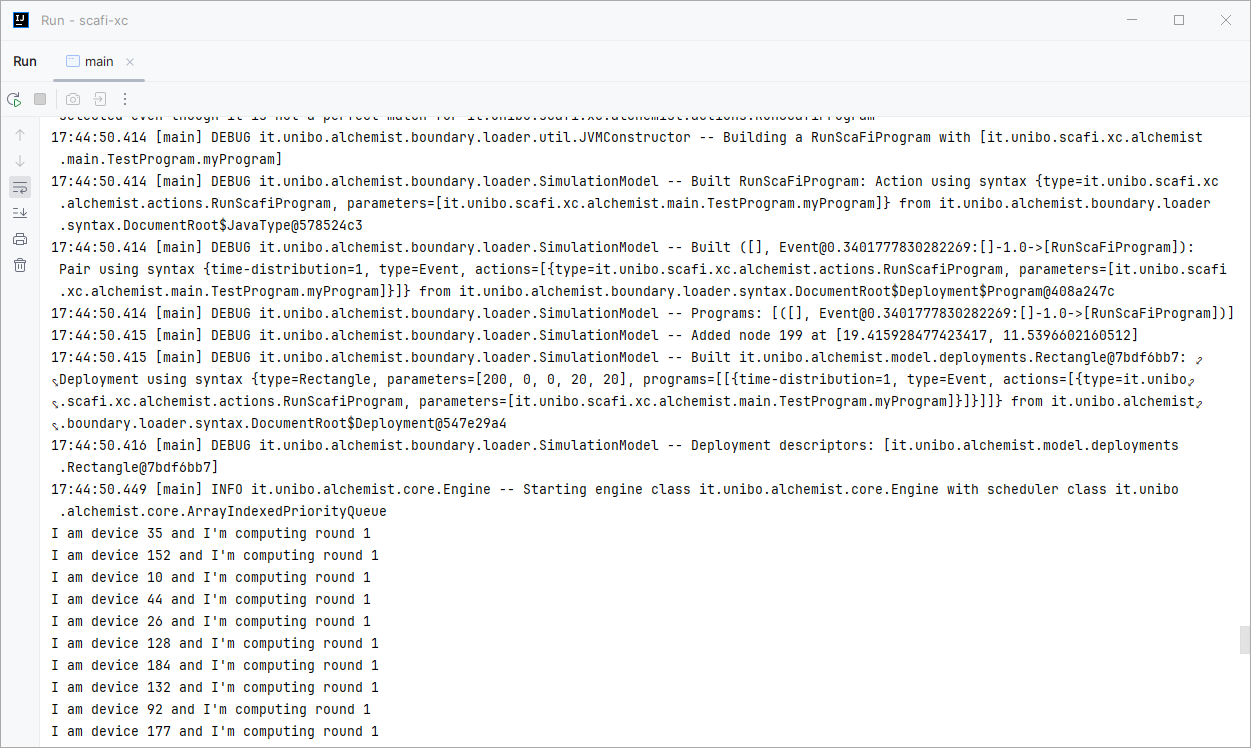
\includegraphics[width=\linewidth]{figures/alchemist-demo.png}
\end{figure}


% ! TeX root = ../thesis-main.tex
%----------------------------------------------------------------------------------------
\chapter{Evaluation}
\label{chap:evaluation}
%----------------------------------------------------------------------------------------

\section{Programming experience evaluation}

TODO

\section{Unit tests}

The unit test framework used for the project is ScalaTest, a popular testing framework for Scala.
%
All the unit tests are defined as traits or classes that depend on a common trait called \texttt{UnitTest}, which provides a common testing \ac{DSL} called \texttt{AnyFlatSpec}, enhanced with the \texttt{ShouldMatchers} trait and other utilities, that make the test assertions look like natural spoken language.
%
Unit tests cover the \texttt{common}, \texttt{core}, and \texttt{simulator} modules.
%
\texttt{UnitTest} is also the base for the \texttt{AcceptanceTest} class of the \texttt{tests} module, to have a consistent testing style across the whole project.

Given that the expected behavior of the aggregate programming libraries \ac{API} strictly relates to the chosen semantics that implements the necessary syntaxes, the unit tests for the libraries are tied to the semantics they are tested with.
%
For the scope of the project, \ac{XC} is the only semantics implemented, so the libraries are tested against it.
%
Unit tests for libraries always include a sample program using the subject under test, and during the test cases, the program is executed in a test environment and inspected, both for the expected results and for the expected value tree produced by the test context.


\section{Acceptance tests}

Acceptance tests are an important validation tool for the project, as they are the only way to ensure that the libraries are working as expected in simulated scenarios.
%
The tests are aimed to be as readable as possible, using the unit test \ac{DSL}, but also hiding all the complexity of the simulation setup and execution.
%
The most important acceptance test currently present is the \texttt{GradientWithObstacleTest}, which is a simulation of a bi-dimensional grid network of devices that compute a gradient from a source, with an obstacle in the middle of the grid that appears halfway through the simulation.
%
The gradient is expected to be recalculated after the obstacle appears, and the test checks that the devices adapt to the new environment.


\section{Continuous Integration} \label{chap:evaluation->sec:continuous-integration}

Both unit and acceptance tests are run automatically by the continuous integration pipeline, built with \textit{GitHub Actions}\footnote{\url{https://github.com/features/actions}} and hosted by GitHub\footnote{\url{https://github.com/ldeluigi/scafi-xc/actions}}.
%
The pipeline is invoked on every push to the repository, and it runs the tests on the latest version of the codebase, as well as on every push on open pull requests, given that \this is meant to be open source, under the \textit{Apache License 2.0}.


\section{Code Style} \label{chap:evaluation->sec:code-style}

Having a consistent and \quotes{clean} coding style across the entire project contributes to the maintainability and readability of the codebase.
%
For this reason, automatic code formatting and linting tools are used to enforce a consistent style across the project.
%
The tools put in place are \textit{scalafmt} and \textit{scalafix}, each with their own configuration file and rule sets, specific for Scala 3.
%
The code style is enforced by two dedicated phases of the continuous integration pipeline, described in \Cref{chap:evaluation->sec:continuous-integration}.


% ! TeX root = ../thesis-main.tex
%----------------------------------------------------------------------------------------
\chapter{Conclusion and Future Work}
\label{chap:conclusion-and-future-work}
%----------------------------------------------------------------------------------------

The objective of this work has been to develop a \ac{DSL} foundation, which would serve as the basis for a new framework named \this.
%
The framework proposed is intended to redesign and improve the ScaFi toolkit, is implemented using the Scala 3 programming language, and is supported by the Exchange Calculus computational model and formal language.
%
The development of \this involved prototyping, interviews, and the application of advanced programming patterns with Scala 3.
%
Continuous integration and acceptance testing were utilized to ensure the quality and reliability of the framework.
%
The requirements for \this, collected through interviews with stakeholders, have all been satisfied, including optional ones, so the final result can be considered a success.
%
However, the current implementation covers only a fraction of the functionality offered by the original ScaFi framework, leaving room for further extensions.

The concrete implementations presented here aim for simplicity, readability, correctness, and reusability, deferring concerns about performance and efficiency for future iterations.
%
Furthermore, the developed simulator offers a very restricted set of features in comparison to the original ScaFi simulator, needing improvements to support more complex scenarios and one or more graphical interfaces for the user to interact with the simulator.
%
The following paragraphs provide a list of possible future developments.

\paragraph{Performance optimization} The current implementation of the context and the simulator is not optimized for performance.
%
For example, the context leverages the \texttt{Map} data structure to represent \texttt{ValueTree}s, which is not the most efficient data structure for this purpose, as it stores multiple copies of all the common prefixes of the keys.

\paragraph{Complete re-implementation of the core module} The \texttt{core} module is the foundation of the ScaFi framework, as it contains the basic building blocks for the development of aggregate programs.
%
In \this, it has been implemented only partially, since the only advanced construct implemented is the gradient.
%
A comprehensive extension to include the full standard library is essential for the framework's completeness.

\paragraph{Enhancements of the simulator} The current simulator does not support many of the features of the original ScaFi simulator and is limited to discrete time.
%
Extensions of the implementation or a complete redesign can provide a more comprehensive feature set, including support for graphical user interfaces.

\paragraph{Support for real-world distributed systems} The original ScaFi allowed the deployment of aggregate programs on real-world distributed systems with the \texttt{spala} and \texttt{distributed} modules, currently absent in \this.
%
Implementing such support is a crucial step to consider \this a valid replacement for the original ScaFi.

\paragraph{Experimental developments with aggregate programming} The reusability and the modularity of the new core module allow it to be extended with new, experimental libraries and semantics, fostering research projects exploring novel aspects of aggregate programming.

\paragraph{Adding more acceptance tests} Most of the reliability of the framework comes from the functionality and readability of its tests.
%
In particular, acceptance tests are designed to be proofreadable by experts in the field, and they are the most important tests for the framework.
%
Nevertheless, only a few acceptance tests are currently present.
%
Strengthening the test suite would enhance the reliability of the framework, ensuring its robustness in a wider range of scenarios.

\paragraph{Improvement of the Alchemist incarnation} The integration with the Alchemist simulator is still a prototype.
%
A more complete implementation would enable more sophisticated simulation scenarios, such as those involving situated agents, with sensors and actuators actively managed by the aggregate program.

\paragraph{Survey evaluation of the framework} A survey evaluation of the framework could be conducted to assess the usability and effectiveness of the framework in the development of aggregate programs.
%
Additionally, it could provide conclusive results regarding the impact of the Context-based constraints on shared values discussed in \Cref{chap:implementation->sec:context-based-constraints}.
%
Whether or not the proposed changes to the core represent a valid improvement is still an open question, and a survey evaluation of the proposal could provide a definitive answer.

In conclusion, while \this marks a significant step towards a new ScaFi framework, there is still much work to be done.
%
With continued development and iteration, it has the potential to significantly contribute to the field of aggregate programming, both as a development framework and as a research tool.


%----------------------------------------------------------------------------------------
% BIBLIOGRAPHY
%----------------------------------------------------------------------------------------

\backmatter

\nocite{*} % comment this to only show the referenced entries from the .bib file

\bibliographystyle{ieeetr}
\bibliography{bibliography}

\end{document}
